% cGENIE User Manual
% 'muffin'' flavor

% Andy Ridgwell
%
% ---------------------------------------------------------------------------------------------------------------------------------
%
% ---------------------------------------------------------------------------------------------------------------------------------

\documentclass[10pt,twoside]{article}
\usepackage[paper=a4paper,portrait=true,margin=2.5cm,voffset=0pt,ignorehead,footnotesep=1cm]{geometry}
\usepackage{graphicx}
\usepackage{hyperref}
\usepackage{paralist}
\usepackage{caption}
\usepackage{float}
\usepackage{wasysym}
\usepackage{seqsplit}

\linespread{1.1}
\setlength{\pltopsep}{2.5pt}
\setlength{\plparsep}{2.5pt}
\setlength{\partopsep}{2.5pt}
\setlength{\parskip}{2.5pt}

\sloppy

\captionsetup[figure]{justification=raggedright}

\title{cGENIE v.0.9 ('muffin') User Manual}
\author{Andy Ridgwell}
\date{\today}

\begin{document}

%=================================================================================================================================
%=== BEGIN DOCUMENT ==============================================================================================================
%=================================================================================================================================

\maketitle

%=================================================================================================================================
%=== CONTENTS ====================================================================================================================
%=================================================================================================================================

\tableofcontents

%=================================================================================================================================
%=== CHAPTERS ====================================================================================================================
%=================================================================================================================================

%---------------------------------------------------------------------------------------------------------------------------------
%--- README blurb ----------------------------------------------------------------------------------------------------------------
%---------------------------------------------------------------------------------------------------------------------------------

\newpage
\section{README blurb}\label{README blurb}

This document covers the directory structure of the source code and ancillary data input files, instructions for compiling the GENIE executable, and how to configure and execute an experiment (i.e., how to get some actual work done). Also covered is how to specify the results you want saved and at what points in time, in what format they are saved, and (some ways of) getting the results visualized.

\noindent A Quick Start Guide is provided in Appendix A (page \pageref{Appendix A}) if you prefer to just jump in semi-blind.
However, it is advisable to at least read the FAQ section, lest any of the FAQs become EMFAQs (Even More Frequently Asked Questions) ...

For additional information refer to the companion \textbf{Tutorial} (\texttt{genie-tutorial}) and \textbf{HOW-TO} (\texttt{cgenie-howto}) documents.
The source for this document is in TEX and resides on the SVN repository under:
\vspace{-5.5pt}\begin{verbatim}
~/cgenie/genie-main/doc
\end{verbatim}\vspace{-5.5pt}

All the documentation (including this) can be generated from the TEX source in both postscript (.ps) and Adobe (.pdf) formats.
To build documentation from the TEX source -- from witin (\texttt{\~{}/genie-main/doc})\footnote{\~{} stands for the home directory}, issue the command\footnote{At the \texttt{\$} prompt}:
\begin{compactitem}
	\item\begin{verbatim}$ make user-manual\end{verbatim}
	Builds the GENIE user manual. [NOW REDUNDANT -- SEE GENIE WIKI]
	\item\begin{verbatim}$ make cgenie-user-manual\end{verbatim}
	Builds the (biogeochemistry and cGENIE focused) user manual.
	\item\begin{verbatim}$ make genie-tutorial\end{verbatim}
	Builds documentation describing various tutorials and example model configurations and experimental designs.
	\item\begin{verbatim}$ make cgenie-howto\end{verbatim}
	The HOW-TO documentation (potted explanations of how to get stuff done).
\end{compactitem}

To clean up previously built documentation:
\begin{compactitem}
	\item\begin{verbatim}$ make clean\end{verbatim}
	Cleans the built user-manual documentation files.
	\item\begin{verbatim}$ make clean-genie clean-cgenie\end{verbatim}
	Cleans all the built files for the genie-* and cgenie-* documentation.
\end{compactitem}

\noindent\textbf{PLEASE edit and update the documentation and populate it with wonderful useful things. Spread the love :o)}

%---------------------------------------------------------------------------------------------------------------------------------
%---------------------------------------------------------------------------------------------------------------------------------

\subsection{Naming conventions blurb}\label{Naming conventions blurb}

The modular Earth system model is called \href{www.genie.ac.uk}{GENIE}, which stands for: Grid ENabled Integrated Earth system model. There are 2 primary variants - one with a simple (2-D, EMBM - see below) atmosphere, which is used here and referred to as 'GENIE-1', and one which employs a 3-D dynamical GCM atmosphere, called GENIE-2. cGENIE is a developmental variant that branches off of the primary model development pathway (the 'trunk') and which reside on 'branches' (all handled by the Subversion (SVN) code repository).

We will assume that the model directory structure (\texttt{cgenie/}), results directory, and (optional) model configuration directory and run scripts all reside in a directory given by \texttt{\~{}}, which may look something like:
\vspace{-5.5pt}\begin{verbatim}
home/username
\end{verbatim}\vspace{-5.5pt}

\noindent where \texttt{\textit{username}} is your username. Model output (the directory where the results of the model experiments will be saved) will then appear here:
\vspace{-5.5pt}\begin{verbatim}
home/username/genie_output
\end{verbatim}\vspace{-5.5pt}
\noindent or
\vspace{-5.5pt}\begin{verbatim}
~/genie_output
\end{verbatim}\vspace{-5.5pt}

Rather than having multiple directories and ancillary files all cluttering up your home directory level and making it look untidy, the everything can be placed at an alternative location, e.g.:
\vspace{-5.5pt}\begin{verbatim}
~/my_model_stuff/genie
\end{verbatim}\vspace{-5.5pt}

To install and run GENIE with a non-standard directory structure, the following files in \texttt{\~{}/genie/genie-main} will have to be edited\footnote{When editing these files, particularly in Windoz, remember that these files must be executable.}:
\vspace{-5.5pt}\begin{verbatim}
user.mak
user.sh
\end{verbatim}\vspace{-5.5pt}

The science modules currently available are listed in Appendix B (page \pageref{Appendix B}).

%---------------------------------------------------------------------------------------------------------------------------------
%---------------------------------------------------------------------------------------------------------------------------------

\subsection{Model background blurb}

The core model component is the climate model C-GOLDSTEIN, as described in \textit{Edwards and Marsh} [2005] (calibrated in \textit{Hargreaves et al.} [2005] with minor bug fixes described in \textit{Ridgwell et al.} [2007a]). It comprises three modules:
\begin{compactitem}
	\item GOLDSTEIN (the 3-D ocean circulation model of \textit{Edwards and Shepherd} [2001])
	\item dynamic-thermodynamic sea-ice, and
	\item 2-D EMBM (Energy-Moisture Balance Model) following \textit{Weaver et al.} [2001].
\end{compactitem}
In GENIE-1 terminology, this EMBM atmosphere plus GOLDSTEIN ocean plus sea-ice (linked to GOLDSTEIN) has the 'flavor' (i.e., specific combination of science modules):
\vspace{-5.5pt}\begin{verbatim}
genie_eb_go_gs
\end{verbatim}\vspace{-5.5pt}

The addition of ocean (and atmosphere) biogeochemistry gives you a coupled climate - carbon cycle model which was called CB-GOLDSTEIN in its non-modular, pre-GENIE incarnation. In addition to the GOLDSTEIN+sea-ice+EMBM flavor; \texttt{genie\_eb\_go\_gs}, CB-GOLDSTEIN has an ocean biogeochemistry module called BIOGEM (for 'BIOGEochemistry Model'), a module to update and keep track of the atmospheric 'chemistry' (greenhouse gas concentration and isotopic composition) called ATCHEM ('ATmospheric CHEmistry Model'), and a coupler to exchange fluxes between ocean and atmosphere across the air-sea interface. The coupler also provides BIOGEM  with information about the overlying atmospheric composition, and if required, can drive the EMBM with trace gas concentrations for calculating radiative forcing of climate. As well as indirect coupling via the atmosphere and EMBM, BIOGEM and GOLDSTEIN are directly coupled through the exchange of 3-D array information regarding the geochemical composition of the ocean. BIOGEM also makes copies of various key configuration parameters at start-up as well as paying attention to sea-ice extent etc, and provides these all as output (independently of GOLDSTEIN ). The GENIE-1 flavor equivalent to CB-GOLDSTEIN is:
\vspace{-5.5pt}\begin{verbatim}
genie_eb_go_gs_ac_bg
\end{verbatim}\vspace{-5.5pt}

The configuration, calibration, and evaluation of GENIE-1, is described in \textit{Ridgwell et al.} [2007a]. Earlier incarnations of the ocean biogeochemistry are described in \textit{Cameron et al.} [2005] and \textit{Lenton et al.} [2006].
The global carbon cycle can be further extended with the addition of a representation of the mass balance of solid material deposited to deep-ocean sediments - a module called SEDGEM ('SEDiment GEochemistry Model'). This is coupled via an interfacing module to BIOGEM. The overall coupled climate-ocean biogeochemistry-sediment geochemistry model was previously termed CBS-GOLDSTEIN, but in GENIE-1 terminology is:
\vspace{-5.5pt}\begin{verbatim}
genie_eb_go_gs_ac_bg_sg
\end{verbatim}\vspace{-5.5pt}

The configuration, calibration, evaluation, and application of GENIE-1 with deep-sea sediments, is described in \textit{Ridgwell and Hargreaves} [2007] and \textit{Ridgwell et al.} [2007b]. Further developments to the sediment model are described in \textit{Ridgwell} [2007].

When allowing burial of biogenic material in deep-sea sediments using the SEDGEM module, a further module is available to provide the (long-term) balance the loss of matter from the ocean. This is called ROKGEM (for: 'ROcK GEochemistry Model') and calculates the solute supply to the coastal ocean resulting from the weathering on land of exposed rock surfaces and soil minerals. The flavor of GENIE run with this additional weathering module is then termed:
\vspace{-5.5pt}\begin{verbatim}
genie_eb_go_gs_ac_bg_sg_rg
\end{verbatim}\vspace{-5.5pt}

The Table ~\ref{fig:genie_modules} in Appendix B summarizes the different science modules in GENIE.

Suggested background readings to help understanding the model, its typical applications, its successes and perhaps more importantly its limitations are:
\begin{compactitem}
	\item \textit{Annan et al.} [2005]
	\item \textit{Edwards and Marsh} [2005] (for the fast climate model core component, C-GOLDSTEIN)
	\item \textit{Edwards and Shepherd} [2001]
	\item \textit{Hargreaves et al.} [2004]
\end{compactitem}
For atmosphere-ocean(-sediment) carbon cycling and biogeochemistry, try:
\begin{compactitem}
	\item \textit{Ridgwell et al.} [2007a,b]
	\item \textit{Ridgwell and Hargreaves} [2007]
	\item \textit{Ridgwell} [2007]
	\item \textit{Cameron et al.} [2005] (for an earlier representation of biogeochemical cycling in the ocean and atmosphere)
	\item \textit{Lenton et al.} [2006]
	\item \textit{Ridgwell} [2001]
	\item \textit{Ridgwell et al.} [2002]
\end{compactitem}

\noindent Versions of most of the relevant model references can either be downloaded from:
\begin{compactitem}
	\item \href{www.genie.ac.uk}{the 'official' GENIE project site}, or
	\item \href{www.seao2.org/pubs.html}{my own publications server}.
\end{compactitem}

\noindent Also refer to the companion documentation to this manual:
\begin{compactitem}
	\item \texttt{genie-tutorial.tex} -- Documentation describing various tutorials and example model configurations and experimental designs.
	\item \texttt{genie-howto.tex and cgenie-howto.tex} --' HOW-TO' documentation (potted explanations of how to get stuff done).
\end{compactitem}

%---------------------------------------------------------------------------------------------------------------------------------
%--- Getting your grubby little mitts on the model -------------------------------------------------------------------------------
%---------------------------------------------------------------------------------------------------------------------------------

\newpage
\section{Getting your grubby little mitts on the model}

First, you will need a copy of Subversion (abbreviated: 'SVN') installed on the machine you want to run the model on (or at least, on the machine you want the source code to be maintained on). See:
\begin{compactitem}
	\item the \href{http://en.wikipedia.org/wiki/Subversion\_(software)}{Wikipedia entry} or
	\item the \href{http://source.ggy.bris.ac.uk/wiki/GENIE\_running\_an\_expt}{GENIE wiki}
\end{compactitem}
for a basic over-view of obtaining the source code (wiki username and password required ...). In summary:

If you are using linux, then you will most likely have the command line client already installed. Try typing:
\vspace{-5.5pt}\begin{verbatim}
$ which svn
\end{verbatim}\vspace{-5.5pt}
to see if the client is in your path. Command line and GUI clients for SVN are available for just about any operating system. \texttt{tortoisesvn} is popular for windows. \texttt{SVNx} is a good choice for the Mac.

Once you have Subversion installed, you will be prompted for your password when required. SVN caches your password, and so you often do not need to type it.

You can get ('check out'\footnote{\texttt{svn co} is synonimous with \texttt{svn checkout}}) a copy of GENIE from SVN by typing:

\vspace{-5.5pt}\begin{verbatim}
$ svn co https://svn.ggy.bris.ac.uk/subversion/genie/branches/cgenie
  --username=genie-user cgenie
\end{verbatim}\vspace{-5.5pt}

To update an existing checkout, simply \texttt{cd} to the highest-level directory (\texttt{\~{}}) and issue the update command:

\vspace{-5.5pt}\begin{verbatim}
$ svn update
\end{verbatim}\vspace{-5.5pt}

\noindent note that you could update just a sub-tree of your checkout by changing directory to, say 
\vspace{-5.5pt}\begin{verbatim}
~/cgenie/genie-embm
\end{verbatim}\vspace{-5.5pt}
and then calling 
\vspace{-5.5pt}\begin{verbatim}
$ svn update
\end{verbatim}\vspace{-5.5pt}
which would result in an updating of just the EMBM module.
Or you could just update a single file with \texttt{svn update \textit{\texttt{filename}}} from within the appropriate directory, or by additionally supplying the path.

%---------------------------------------------------------------------------------------------------------------------------------
%---------------------------------------------------------------------------------------------------------------------------------

\subsection{Where am I ... ? (what is in the file-tree?)}

The pertinent directories associated with configuring and running experiments with the carbon cycle and (EMBM-based) climate using cGENIE are listed in full in Appendix C (page \pageref{Appendix C}).

%---------------------------------------------------------------------------------------------------------------------------------
%---------------------------------------------------------------------------------------------------------------------------------

\subsection{Configuring GENIE for your local software environment}

Some hints for instally and adapting GENIE for your local software environment (and machine architecture) can be found in the documents \texttt{README} and \texttt{readme.main} in \texttt{\~{}/genie-main/docs}
\noindent but note that they are specific to GENIE (not genie) and refer to CVS rather than SVN for code repository access (as well as some other out-of-date details). no doubt these will be updated in due course ...

A general GENIE user-manual can also be created in a variety of formats (including .ps and .pdf) from within \texttt{\~{}/genie/genie-main/doc} by issuing the command:
\vspace{-5.5pt}\begin{verbatim}$ make user-manual\end{verbatim}\vspace{-5.5pt}
\noindent However, this currently suffers from some of the same documentation issues as the ASCII files in genie-main is as much as it is specific to GENIE (trunk) and assumes use of a CVS (rather than SVN) code repository. Again, an update will follow ... (ha ha ha ha)

%---------------------------------------------------------------------------------------------------------------------------------
%--- Running GENIE ---------------------------------------------------------------------------------------------------------------
%---------------------------------------------------------------------------------------------------------------------------------

\newpage
\section{Running cGENIE}

I'll discuss this in the reverse order just for the hell of it -- setting a model experiment going \textit{first} ... and only then describing what you should have done in the first place to have set it up correctly ;)

It is important to recognize from the onset that there are two fundamental modes of operating cGENIE - as a new or continuing run. A new run is one which starts off from a default state of the system.
\begin{compactitem}
	\item In the case of the ocean model GOLDSTEIN, this is with the ocean set to uniform temperature and salinity throughout\footnote{See HOWTO for details of how to initialize with non-uniform initial T and S distributions.}, and no momentum.
	\item In BIOGEM, the dissolved tracers are initialized with default values applied to all wet cells while all particulate concentrations in the ocean are zero.
	\item In ATCHEM all tracer gas concentrations (and isotopic properties) are initialized with uniform default values everywhere in the atmospheric grid.
	\item In SEDGEM the sediments are set to a homogeneous (detrital or ash tracer) composition throughout.
\end{compactitem}
	A continuing run will carry on from where-ever a previous run left off, using a set of files called 'restart' files that between them completely define a snapshot state of the system. More on this (plus examples) later (and in the tutorial document).
	
For \textit{c}GENIE, a model experiment can be initiated in two different ways ...

%---------------------------------------------------------------------------------------------------------------------------------
%---------------------------------------------------------------------------------------------------------------------------------

\subsection{... manually ... :(}

The basic flavor and configuration of cGENIE is run from \texttt{\~{}/cgenie/genie-main} by typing:
\vspace{-5.5pt}\begin{verbatim}./genie_example.job\end{verbatim}\vspace{-5.5pt}
\noindent \texttt{genie\_example.job} is a shell script which sets up a basic ('base') configuration of the model. A different flavor and configuration of the model is enabled by specifying an alternative base configuration file:
\vspace{-5.5pt}\begin{verbatim}./genie_example.job -f another.config\end{verbatim}\vspace{-5.5pt}
where \texttt{another.config} is a specified model configuration (/flavor) \texttt{.config file}.

cGENIE is supplied with a number of pre-prepared \textit{base config} files. These live in:
\vspace{-5.5pt}\begin{verbatim}
~/cgenie/genie-main/configs
\end{verbatim}\vspace{-5.5pt}
The names of the \textit{base config} files are typically structured as:
\vspace{-5.5pt}\begin{verbatim}
genie_aa_oo_ss_xxxx.config
\end{verbatim}\vspace{-5.5pt}
where:

\begin{compactitem}

	\item \texttt{aa} is the atmosphere name (\texttt{ig}=igcm, \texttt{eb}=embm)
	
	\item \texttt{oo} is the ocean name (\texttt{fi}=fixed, \texttt{go}=goldstein ocean, \texttt{sl}=slab)
	
	\item \texttt{ss} is the sea-ice name (fi=fixed,gs=goldstein seaice, sl=slab), and
	
	\item xxxx is for any more info (e.g., \texttt{ac}=ATCHEM, \texttt{bg}=BIOGEM, \texttt{sg}=SEDGEM, \texttt{rg}=ROKGEM).
	
\end{compactitem}

A relatively simple configuration file is \texttt{genie\_ig\_fi\_fi.config} -- a dynamical atmosphere (IGCM) plus prescribed ocean surface and sea-ice boundary conditions. In addition to specifying the flavor and grid resolution, this configuration file also changes the run-length from one month to 10 years and turns on daily IGCM atmosphere output. It also changes the name of the directory in which the experimental output is placed. 

%---------------------------------------------------------------------------------------------------------------------------------
%---------------------------------------------------------------------------------------------------------------------------------

\subsection{... via a shell script :)}

For configuring and running experiments interactively or submitting jobs to a cluster queue, an executable shell script called \texttt{runcgenie.sh} (similar to \texttt{old\_rungenie.sh} before. `CC' means it includes climate and the (ocean) carbon cycle. By default it has 96 time steps per year compared with a 100 previously.
-- \texttt{runcgenie.sh} is held under svn and resides in the directory \texttt{\~{}/cgenie/genie-main}, from where experiments are run.
 Note the file \texttt{runcgenie.sh} \textbf{MUST} have executable permissions (\texttt{chmod u+x runcgenie.sh}).

\begin{compactitem}

        \item   For running cGENIE via the `\texttt{runcgenie.sh}' script, you must create the following two directories:
\end{compactitem}
  \vspace{-5.5pt}\begin{verbatim}
	   ~/cgenie_archive
   ~/cgenie_log
  \end{verbatim}\vspace{-11pt}
(\texttt{\~{}/cgenie\_output} directory is automatically created after issueing the `make assumedgood' command).

\begin{compactitem}

	\item	No new path needs to be specified for `forcings' as these now live in \$/cgenie/genie-forcings, and hence no full path needs to be specified in a `user config' -- just the forcing name on its own. A complete command line now looks like:

	
\end{compactitem}

%---------------------------------------------------------------------------------------------------------------------------------
%---------------------------------------------------------------------------------------------------------------------------------

\subsection{Using \texttt{runcgenie.sh}}

You use \texttt{runcgenie.sh}to run cGENIE, taking example flavor \texttt{cgenie\_eb\_go\_gs\_ac\_bg\_itfclsd\_16l\_JH\_BASEFe} and experiment design (configuration patch file) \texttt{EXAMPLE\_worjh2\_Fe\_SPIN}) as follows:
\vspace{-5.5pt}\begin{verbatim}$ ./runcgenie.sh <options>\end{verbatim}\vspace{-11pt}

\textbf{Now pay attention}: there are 4 (FOUR) parameters that \textbf{must} be passed to the script as \texttt{<options>}:

\begin{compactenum}

	\item The name of the required flavor and basic configuration, but omitting the '\texttt{.config}' bit, e.g.\footnote{Please note that \textit{this is an example}, and does not necessarily mean that this is the same \texttt{.config} file as you want to use ...}:
	\begin{verbatim}cgenie_eb_go_gs_ac_bg_itfclsd_16l_JH_BASEFe\end{verbatim}
	
	\item Path to user (experiment) configuration file (i.e., the file containing the list of namelist changes for a particular experiment). In the example, this looks like:
	\begin{verbatim} / \end{verbatim}
	
	\item The name of the experiment, and specification of \textit{user config} file is to be used, i.e.:
	\begin{verbatim}EXAMPLE_worjh2_Fe_SPIN\end{verbatim}

	\item The run length of the experiment \textbf{in years}\footnote{This must be entered on the command line as an integer, even though GENIE will be treating it as a real.}.

\end{compactenum}

A typical command line to run the model might thus look something like (all one line and be careful with the S P A C E S):
\vspace{-5.5pt}\begin{verbatim}./runcgenie.sh cgenie_eb_go_gs_ac_bg_itfclsd_16l_JH_BASEFe
 / EXAMPLE_worjh2_Fe_SPIN 10001\end{verbatim}\vspace{-5.5pt}

	5. The full path (and name) of any restart required\footnote{There must exist a subdirectory in \texttt{\~{}/cgenie\_output} with this name.}.

\noindent If the 5th (optional) parameter is not passed then GENIE will run from 'cold' (i.e., no re-start). If the 5th parameter is present then GENIE will attempt to run from a previously generated re-start state.

A typical command line to run the model using a specified re-start might thus look something like (all one line):
\vspace{-5.5pt}\begin{verbatim}./runcgenie.sh cgenie_eb_go_gs_ac_bg_itfclsd_16l_JH_BASEFe
 / EXAMPLE_worjh2_Fe_SPIN 10001 cgenie_eb_go_gs_ac_bg.xx\end{verbatim}\vspace{-5.5pt}
in which the experiment \texttt{EXAMPLE\_worjh2\_Fe\_SPIN} will be run for 10001 years, using the flavor and basic configuration specified by \texttt{cgenie\_eb\_go\_gs\_ac\_bg\_itfclsd\_16l\_JH\_FeBASE}, and using as a restart, the experiment saved in this location:
\vspace{-5.5pt}\begin{verbatim}~/genie_output/cgenie_eb_go_gs_ac_bg.xx\end{verbatim}\vspace{-5.5pt}

In this methodology, for each model experiment you will require a plain text (ASCII) file that details any namelist parameter changes compared to the GENIE defaults and the basic flavor and configuration defined in the \texttt{.config} file. If you require any tracer forcings then you will also need to specify the directory containing the necessary forcing specification files . The location of the directory where GENIE will go looking for forcing specification files is set by a namelist parameter (\texttt{bg\_par\_forcing\_name}). Full details of the specification and application of tracer forcings is given later.

\noindent Full details regarding what \texttt{runcgenie.sh} actually does can be found in Appendix E (page \pageref{Appendix E}).

\begin{figure}[h]
\includegraphics*{genie_expflowchart.eps}
\caption{Schematic of the sequence-of-events in configuring and running an experiment using the \texttt{runcgenie.sh} methodology.}
\label{fig:genie_expflowchart}
\end{figure}

%---------------------------------------------------------------------------------------------------------------------------------
%---------------------------------------------------------------------------------------------------------------------------------

\subsection{Job submission to a cluster}

For submitting jobs with Sun Grid Engine (SGE) on a cluster:\footnote{With a different queue management environment it may be necessary to place the call to \texttt{genie.sh} together with its list of parameters into an executable shell, and submit that instead. }:
\vspace{-5.5pt}\begin{verbatim}$ qsub -S /bin/bash subgenie.sh <options>\end{verbatim}\vspace{-5.5pt}
Here: the \texttt{-S /bin/bash} part is to ensure that SGE uses the BASH shell to submit the job because this is the language that \texttt{subCCgenie.sh} has been written in.

Take care that the installed FORTRAN compiler can be seen by the cluster nodes. If not, the GENIE executable must have already been built prior to submitting a job. The easiest way to do this is to run GENIE interactively briefly (e.g., with a run length of just a couple of years or kill it) and then submit the full run to the cluster.

Other useful submission options for SGE:

\begin{compactitem}

	\item To redirect the standard output stream:
	\vspace{-5.5pt}\begin{verbatim}$ qsub -o genie_log ...\end{verbatim}
	
	\item To redirect the standard error stream:
	\vspace{-5.5pt}\begin{verbatim}$ qsub -e genie_log ...\end{verbatim}
	
	\item To merge standard output and error streams into standard output:
	\vspace{-5.5pt}\begin{verbatim}$ qsub -j y ...\end{verbatim}
	
	\item To specify particular resources, such as the nodes with 8 GB of RAM:
	\vspace{-5.5pt}\begin{verbatim}$ qsub -l mem_total = 8.0G ...\end{verbatim}
	
	\item To decrease the priority of a job\footnote{The default priority is 0. A lower priority has a higher value ... !}:
	\vspace{-5.5pt}\begin{verbatim}$ qsub -p 1 ...\end{verbatim}
	
	\item To submit a job from the current working directory:
	\vspace{-5.5pt}\begin{verbatim}$ qsub �cwd\end{verbatim}
	
	\item Request an email is sent when the job starts and/or when it finishes -- see the main pages for \texttt{qsub} for the required syntax).
	
	\item A complete example would be:
	\vspace{-5.5pt}\begin{verbatim}$ qsub -q kitten.q -j y -o genie_log -S /bin/bash runcgenie.sh
        genie_eb_go_gs_ac_bg / epx1_modern 51 <options>\end{verbatim}
	which merges standard output and error streams and redirects the resulting file to the directory \~{}/cgenie\_log.
	Note that to redirect output as per in this particular example, the directory \texttt{\~{}cgenie\_log} \textbf{MUST} be present. I have no idea what happens if it is not ... but it can't be good ;)
	
\end{compactitem}

\noindent You can check the status of the SGE job queue with the command:
\vspace{-5.5pt}\begin{verbatim}$ qstat -f\end{verbatim}\vspace{-5.5pt}
and you can kill a job with the \texttt{qdel} command, the job numbers being given by the \texttt{qstat} command.

On \texttt{almond.ggy.bris.ac.uk} you can graphically check what is going on via the www. In an X window, enter:
\vspace{-5.5pt}\begin{verbatim}$ ssh almond.ggy.bris.ac.uk
$ firefox --no-remote &\end{verbatim}\vspace{-5.5pt}
and follow the links: 'Cluster Status (Ganglia)', and then 'Job Queue' to get to the actual queue listing and cluster status.

\noindent \textbf{NOTE}: It is common on clusters for the FORTRAN compiler to not be accessible by the computer nodes. \texttt{almond.ggy.bris.ac.uk} is no exception in this. The implication of this is that \textbf{the GENIE-1 modules must be already compiled BEFORE a job is submitted to the queue}.

\noindent In other words; if you have just issued a \texttt{make cleanall}, you MUST briefly run your desired experiment (or equivalent) interactively (i.e., in the shell window) to ensure that everything is correctly compiled. For instance, either run the experiment for 1 or 11 years say, or (better): start the experiment for the desired full duration, but 'kill it' (Ctrl-C) once the experiment is running successfully.

\noindent Remember that if you have just changed model resolution or number of tracers you must force a complete recompile by issuing a \texttt{make cleanall} (and then start the model running interactively in a shell).

%---------------------------------------------------------------------------------------------------------------------------------
%--- Specifying time-dependent changes to tracer concentrations ('forcings') -----------------------------------------------------
%---------------------------------------------------------------------------------------------------------------------------------

\newpage
\section{Specifying time-dependent changes to tracer concentrations ('forcings')}

Even the most highly coupled instance of GENIE is far from being a complete description of the Earth system. For instance, the lack of a dynamic atmosphere able to perform tracer advection means that dust deposition to the ocean surface cannot be internally calculated. With respect to longer-term biogeochemical cycling, the model currently lacks any explicit representation of shallow water carbonate deposition in banks and reefs. In terms of global change and anthropogenic impacts on carbon cycling and climate, GENIE is also unable to predict fossil CO2 emissions from human activities (just how much do you want to burn in the future?). Provision is therefore made for prescribing flux fields or boundary conditions to the model. These are termed forcings.

There is a serious difficulty in devising a means for implementing a boundary condition to the model because the most interesting and relevant forcings tend to be time-dependent (i.e., the magnitudes vary with time). Worse, the boundary conditions are often spatially heterogeneous (i.e., the magnitude of the forcing is not the same at each and every grid point or cell). Dust fluxes are a good example of spatial heterogeneity in a flux input to the system. To fully define a time-varying 2D flux forcing for say 1000 years of model integration at a 0.01 yr time-step equates to \begin{math}36\times36\times1000\times100\end{math} data points -- clearly beyond simple and efficient data manipulation and processing. One end-member solution would be to define the complete spatial distribution, but leave the fluxes invariant with respect to time. The opposite end-member would by to fully define the time-varying nature of the forcing but distribute the flux uniformly in space. Both approaches have serious drawbacks for many applications. A compromise scheme has therefore been devised to encapsulate data input and output as efficiently and as flexibly as possible.

Firstly, the forcing of atmosphere, ocean, and sediment tracers are treated separately. For the atmosphere (\texttt{atm\_*}) tracers, atmospheric composition is manipulated from the 2-D surface ocean grid of BIOGEM. This means that no forcing is applied to the atmosphere overlying 'dry' land cells. For the ocean (\texttt{ocn\_*}) tracers, all the 'wet' cells in of the full 3-D ocean grid of BIOGEM can be forced. For the sediment (\texttt{sed\_*}) tracers, all the cells comprising the 3-D ocean grid of biogem (rather than the 2D SEDGEM grid) are manipulated\footnote{No provision is currently made for restoring forcing.}.

Secondly, two different types of \textit{forcings} of the system are recognized: a flux forcing and a restoring forcing. The first type, the flux forcing, is pretty self-evident - it represents a flux of tracer that is applied to each cell. The restoring forcing is less intuitive -- a flux is applied to the grid cells with a value calculated to bring the tracer values closer to the prescribed restoring value. A time-scale (in years) determines the rate at which the tracer values are brought toward the boundary condition. This time-scale value is termed the restoring constant. The smaller the value of the restoring constant the 'harder' the restoring, and the more rapidly the model will be constrained to approach the boundary condition.

Whether a flux or restoring forcing is required together with the details of the forcing, and what tracer(s) is (/are) to be forced, are specified in a set of 3 tracer forcing configuration files; one for each type of tracer:

\begin{compactitem}

	\item \texttt{configure\_forcings\_atm.dat}
	
	\item \texttt{configure\_forcings\_ocn.dat}
	
	\item \texttt{configure\_forcings\_sed.dat}
	
\end{compactitem}

Each file consists of rows of settings; one row for each different tracer. The settings are arranged into columns; the description of each column and allowed values are summarized at the bottom of each file. Options include whether a flux or restoring forcing is required, the time-constant of any restoring forcing, etc.

For a tracer forcing top be fully defined, one further set of files are required, taking filenames of the format:

\begin{compactitem}

	\item \texttt{biogem\_force\_*\_sig.dat}
	
\end{compactitem}

\noindent and contains two columns of information: the first is a time marker (year) and is paired with a corresponding tracer scalar  value in the second column. These files all live happily together in the directory defined by the namelist parameter: (\texttt{i,j}).
The information in the signal file define the time-varying information. For a model year falling outside of the maximum or minimum time markers specified in the signal file, no forcing will be applied (this in effect allows a restoring forcing to be turned 'on' and then 'off' again later). For model years inbetween specified time points, the tracer scalar values are linearly interpolation. It should be noted that \texttt{biogem\_force\_*\_sig.dat} file must contain at least one (row) entry.

The units for the flux forcing for all tracers is mol yr-1 for bulk fluxes, and per mil for isotopic composition.
For restoring forcings, the units are atmospheres (atm) for atmospheric (gaseous) tracers, and mol kg-1 for ocean (dissolved) tracers. For isotopic tracers, the units are per mil (\permil).

There are then two alternative ways of providing the final information needed to fully describe a tracer forcing -- the spatial component -- by explicitly defining 2- or 3-D distributions (the sole, original methodology), or by assuming a much simpler, point source, or uniform distribution. The latter is rather easier to grasp and implement, but lack the flexibility of the former.

A variety of example tracer \textit{forcing} configurations are provided in (\texttt{genie-forcings}).

%---------------------------------------------------------------------------------------------------------------------------------
%---------------------------------------------------------------------------------------------------------------------------------

\subsection{Tracer forcing as an explicit 2/3-D distributions}

The tracer forcing in the explicit 2/3-D methodology requires two further files, with filenames:

\begin{compactitem}

	\item \texttt{biogem\_force\_*\_I.dat}
	
	\item \texttt{biogem\_force\_*\_II.dat}
	
\end{compactitem}

\noindent These hold information about spatial distributions. The data format of these is either 2-D for the atmosphere or surface ocean only - rows (\texttt{j}) and columns (\texttt{i}), or 3-D (for the whole ocean) with the successive depth layers (\texttt{k}) repeated as \texttt{(i,j)} blocks down through the file.

The way in which these three files are employed to define a spatially-explicit time-varying input field is as follows. The first field file (\texttt{*\_I.dat}) defines the baseline distribution and the second (\texttt{*\_II.dat}) an alternative distribution. The difference between the two fields defines the spatial component of a time-varying forcing. The tracer scalar value in the signal file modifies the difference between the two spatial fields.

Putting it another way -- the magnitude of the forcing that is applied at any location (\texttt{i,j}) and at point in time (\texttt{t}), \begin{math}F_{(i,j),(t)}\end{math}, is equal to the baseline field, defined in \begin{math}biogem\_force\_*\_I_{(i,j)}\end{math}, plus the time-dependent modifier (\begin{math}S_{(t)}\end{math}) times the difference between the two fields, i.e.:

\begin{math}
	F_{(i,j),(t)} = biogem\_force\_*\_I_{(i,j)} + S_({t)} \times \left(biogem\_force\_*\_II_{(i,j)}  - biogem\_force\_*\_I_{(i,j)} \right)
\end{math}

\noindent Remember that the value of the time-dependent tracer scalar (\texttt{S(t)}) is interpolated from the contents of the forcing signal file \texttt{biogem\_force\_*\_sig.dat}.

Because what I have just written above is probably vanishingly indistinguishable from complete gobbledygook, a couple of examples might help (or not):

\begin{compactenum}

	\item One way of using the forcing functionality of BIOGEM would be to assign a minimum forcing field to \texttt{I}, a maximum forcing field to \texttt{II}, and specify a normalized (i.e., taking values between 0.0 and 1.0) series of modifier values in the the signal file. For example, one could continually vary the surface temperature field seen by the marine carbon cycle over the deglacial transition, based on available end-member reconstructions for glacial maximum and modern [\textit{CLIMAP}, 1980]) and by assuming a semi-representative (normalized) signal with which to interpolate between these two time-slice reconstructions (see \textit{Ridgwell} [2001]).
	
	\item A second way of using the functionality of tracer forcing in BIOGEM would be to set every �wet� cell in \texttt{biogem\_force\_*\_I.dat} to a value of 0.0, and every corresponding location in \texttt{biogem\_force\_*\_II.dat} to a value of 1.0. The forcing applied to the model will then be the same as applying the value of the interpolated tracer scalar (in the signal file) equally to each and every cell, i.e.:
	
\begin{math}
	F_{(i,j),(t)} = 0 + S_({t)} \times \left(biogem\_force\_*\_II_{(i,j)}  - 0 \right)
\end{math}

An example of this usage would be in applying a spatially uniform time-varying change in atmospheric composition, such as restoring atmospheric CO2 to an observed historical or predicted future atmospheric concentrations trajectory.
	
\end{compactenum}

It should be noted that although this scheme is generic and can equally be applied to any tracer (\texttt{atm}, \texttt{ocn}, or \texttt{sed} and including isotopic properties) as well as offering reasonable flexibility in representing the time-varying characteristics of a boundary condition, it does have limitations and cannot cover all possible eventualities. For instance, historical changes in atmospheric CFC concentrations and CO2 radiocarbon activity vary not only with time, but the spatial heterogeneity changes in a complex way that cannot be represented as a interpolation between two alternative end-member distributions. In this way the built-in framework for tracer \textit{forcings} in GENIE does not conform to the OCMIP protocol [REF] for ocean (carbon cycle) model evaluation.

%---------------------------------------------------------------------------------------------------------------------------------
%---------------------------------------------------------------------------------------------------------------------------------

\subsection{Tracer forcing as a point source or uniform distribution}

While the spatial forcing fields (\texttt{biogem\_force\_*\_I.dat}, \texttt{biogem\_force\_*\_I.dat}) provide maximum flexibility, they are not always so easy to use, nor perhaps, understand(!) ;)  An alternative, simply way of specifying forcings has therefore been implemented. You can access this by adding the namelist:
\vspace{-5.5pt}\begin{verbatim}
bg_ctrl_force_oldformat=.false.
\end{verbatim}\vspace{-5.5pt}
which simply tells BIOGEM to expect a new file format for the tracer forcing configuration files.

As before, the tracer forcing configuration files live in the directory specified by the namelist parameter
\texttt{bg\_par\_forcings\_name} e.g.:
\vspace{-5.5pt}\begin{verbatim} 
bg_par_forcings_name="worbe2_historical"
\end{verbatim}\vspace{-5.5pt}

There are 3 files - one for each type of tracer (i.e., gas, dissolved, solid/particulate):

	\begin{compactitem}
		
		\item \texttt{configure\_forcings\_atm.dat} -- gases
		
		\item \texttt{configure\_forcings\_ocn.dat} -- dissolved substances
		
		\item \texttt{configure\_forcings\_sed.dat} -- solid substances / particulates
		
	\end{compactitem}
	
For instance, the format of the tracer forcing configuration file \texttt{configure\_forcings\_atm.dat} looks like:

\vspace{-5.5pt}\begin{verbatim}
 01 02   03 04 05 06  07  08
 \/ \/   \/ \/ \/ \/  \/  \/

-START-OF-DATA-
 F  0.0  F  F  F   2  01  01  '[surface air temperature (K)]'
 F  0.0  F  F  F   2  01  01  '[specific humidity (n/a)]'
 f  0.1  f  t  F   2  01  01  '[carbon dioxide (CO2) partial pressure (atm)]'
 f  0.1  f  t  F   2  01  01  '[d13C CO2 (o/oo)]'
 F  1.0  F  F  f   2  01  01  '[oxygen (O2) partial pressure (atm)]'
 F  1.0  F  F  F   2  01  01  '[d18O O2 (o/oo)]'
 F  1.0  F  F  F   2  01  01  '[nitrogen (N2) partial pressure (atm)]'
 F  1.0  F  F  F   2  01  01  '[d15N N2 (o/oo)]'
 F  1.0  F  F  F   2  01  01  '[methane (CH4) partial pressure (atm)]'
 F  1.0  F  F  F   2  01  01  '[d13C CH4 (o/oo)]'
 F  1.0  F  F  F   2  01  01  '[d14C CH4 (o/oo)]'
 F  1.0  F  F  F   2  01  01  '[sulphur hexafloride (SF6) partial pressure (atm)]'
 F  1.0  F  F  F   2  01  01  '[nitrous oxide (N2O) partial pressure (atm)]'
 F  1.0  F  F  F   2  01  01  '[d15N N2O (o/oo)]'
 F  1.0  F  F  F   2  01  01  '[hydrogen sulphide (H2S) partial pressure (atm)]'
 F  1.0  F  F  F   2  01  01  '[d32S of H2S (o/oo)]'
 f  0.1  F  F  F   2  01  01  '[CFC-11 partial pressure (atm)]'
 f  0.1  F  F  F   2  01  01  '[CFC-12 partial pressure (atm)]'
-END-OF-DATA-

 /\ /\ /\   /\ /\ /\  /\  /\  /\
 01 02 03   04 05 06  07  08  09
\end{verbatim}\vspace{-5.5pt}

The description of each column is detailed at the bottom of the file:

\vspace{-5.5pt}\begin{verbatim}
COLUMN #01: include restoring forcing of tracer? [DATA FORMAT: 'T'/'F' ('t'/'f')]
COLUMN #02: time constant of restoring forcing (years) [DATA FORMAT: real]
COLUMN #03: include flux forcing of tracer? [DATA FORMAT: 'T'/'F' ('t'/'f')]
COLUMN #04: scale flux forcing of tracer? [DATA FORMAT: 'T'/'F' ('t'/'f')]
COLUMN #05: force ocean surface in equilibrium with atmosphere?
            (needs ocean restoring forcing set) [DATA FORMAT: 'T'/'F' ('t'/'f')]
COLUMN #06: make forcing uniform over this dimension
            (2 = 2D, 0 = point, ELSE spatially explicit forcing) [DATA FORMAT: integer]
COLUMN #07: i grid location of point forcing [DATA FORMAT: integer]
COLUMN #08: j grid location of point forcing [DATA FORMAT: integer]
COLUMN END: TRACER DESCRIPTION
\end{verbatim}\vspace{-5.5pt}

The columns pertinent to the this alternative way of implementing tracer forcings are:

	\begin{compactitem}
		
		\item \texttt{\#01} - do you want to restore atmospheric composition toward a specified concentration (or isotopic ratio)? '\texttt{t}' for true ('yes'); '\texttt{f}' for false ('no'). Note that it does not matter whether you use upper-case (capitals) ('\texttt{T}') or lower-case ('\texttt{t}'). If selected, column \texttt{\#2} determines the time-constant of the restoring.
		
		\item \texttt{\#03} - (if not \texttt{\#1}) do you want to apply a flux of gas to the atmosphere?
		
		\item \texttt{\#06} - what degree of homogenization of the flux do you wish to apply? '\texttt{2}' == apply flux evenly throughout the atmosphere; '\texttt{0}' apply the flux at a single point only; ('\texttt{-1}' == use the original (more complex) flux forcing methodology with the flux or fractional weighting of total flux specified explicitly at each individual grid point). If 0, a forcing-at-a-point, the next 2 columns (\texttt{\#7} and \texttt{\#8}) then define the (\texttt{i,j}) location on the model grid (longitude ('\texttt{i}') and latitude ('\texttt{j}')) of the point source.
		
	\end{compactitem}

The forcing configuration files for dissolved tracers (\texttt{configure\_forcings\_ocn.dat}) and particulates (\texttt{configure\_forcings\_sed.dat}) should be self-explanatory; again there is a description of each column at the bottom of the file. However, for dissolved tracer forcings, there is an additional column for the '\texttt{k}' (depth level in the ocean) location of a flux applied at a single point, in addition to longitude ('\texttt{i}') and latitude ('\texttt{j}').

%---------------------------------------------------------------------------------------------------------------------------------
%--- Saving data -----------------------------------------------------------------------------------------------------------------
%---------------------------------------------------------------------------------------------------------------------------------

\newpage
\section{Saving data}

This section covers how to generate results files from the model runs, and what file is which and which contains what, and specifically:

\begin{compactenum}
	\item Types of model output.
	\item '\textit{Time-series}' output.
	\begin{compactitem}
		\item \textit{Time-series} file naming conventions.
		\item Specifying which data fields to be saved as \textit{time-series}.
		\item Specifying frequency and timing of \textit{time-series} data saving.
		\item Seasonal/monthly data saving.
	\end{compactitem}
	\item '\textit{Time-slice}' output.
	\begin{compactitem}
		\item \textit{Time-slice} file naming conventions.
		\item Specifying which data fields to be saved as \textit{time-slice}.
		\item Specifying frequency and timing of \textit{time-slice} data saving.
	\end{compactitem}
\end{compactenum}

All results files are saved in module-specific results directories. So, for BIOGEM results files you will need to go to \texttt{\~{}/cgenie\_output/\$RUNID/biogem}, where \texttt{\$RUNID} is the model experiment name, and for SEDGEM results: \texttt{\~{}/cgenie\_output/\$RUNID/sedgem}, etc etc. Note that ATCHEM currently does not save its own data files (which are instead saved by BIGOEM by accessing the atmospheric composition information placed on the surface-atmosphere tracer array). 

Confused? you soon will be ...

%---------------------------------------------------------------------------------------------------------------------------------
%---------------------------------------------------------------------------------------------------------------------------------

\subsection{'Types of model output'}

The results of experiments are written to the directory:
\vspace{-10pt}\begin{verbatim}~/cgenie_output\end{verbatim}\vspace{-10pt}
For any particular experiment, all sub-directories of results, plus copies of input parameters and the model executable, are gathered together in a directory that is assigned the same name as the experiment (== \textit{user-config} file name), e.g.:
\vspace{-10pt}\begin{verbatim}exp1_modern\end{verbatim}\vspace{-10pt}
Every science module then saves its own results in its own sub-directory. So for BIOGEM output, the results files will thus be found in:
\vspace{-10pt}\begin{verbatim}~/cgenie_output/exp1_modern/biogem\end{verbatim}\vspace{-10pt}
Note that ATCHEM does not save its own results (BIOGEM can save information about atmospheric composition and air-sea gas exchange) while SEDGEM essentially saves results only at the very end of a model experiment (BIOGEM can also save the spatial distribution of sediment composition as time-slices as well as mean composition as a time-series). Furthermore, in order to attain a common format for both ocean physical properties and biogeochemistry, BIOGEM can save a range of ocean results in addition to temperature and salinity, such as: velocities, sea-ice extent, mixed layer depth, convective frequency, etc. Also note that SEDGEM saves data only at the end of an experiment\footnote{With the exception of sediment core location environmental properties, which is saved whenever the sediment column grows or contracts (by a 1 cm unit).}, and does not have access to the time-series and time-slice information available to BIOGEM (or even the current 'time' during an experiment) by default. Setting \texttt{sg\_ctrl\_timeseries\_output=.TRUE.} gives the sedgem results (\texttt{seddiag\_misc\_DATA\_GLOBAL}) in files corresponding to the times set with \texttt{sg\_par\_output\_years\_file\_0d} (\texttt{genie-sedgem/data/input/sedgem\_output\_years\_0d.dat} by default).

Saving full spatial distributions for any or all of the tracers at each and every time-step is not practical, not only in terms of data storage but also because of the detrimental effect that repeated disk access has on model performance. Instead, BIOGEM saves the full spatial distribution of whatever tracer, flux, and/or physical properties of the system are required (how what fields are 'required' is specified is discussed later), only at one or more predefined time points (in years). These are called '\textit{time-slices}'. However, rather than taking an instantaneous snapshot, the time-slice is constructed as an average over a specified integration interval.
The second main data format for model output is that of a '\textit{time-series}' of change in a single (integrated) property of the Earth system. Model characteristics must be reducible to a single meaningful variable for this to be practical (i.e., saving the time-varying nature of 3-D ocean tracer distributions is not). Suitable reduced indicators include: the total inventories in the ocean and/or atmosphere of various tracers (or equivalently, the mean global concentrations / partial pressures, respectively), global sea-ice coverage. Like \textit{time-slices}, the data values saved in the time-series files represent averages over a specified integration interval.

For BIOGEM, at the end of an experiment\footnote{Many of the results files are created during initialization and are periodically updated (appended to) during the experiment. Even before the experiment has finished, they may contain data that is useful to view.} some or all of the following files will be present:

\begin{compactenum}
	\item \texttt{fields\_biogem\_2d.nc} -- 2-D fields of (mostly) ocean bottom, ocean surface, and sediment surface properties.\footnote{The mid-points at which time-slices are saved are specified as described above.} Also: water-column integrals of certain geochemistry diagnostics, air-sea gas exchange fluxes, atmospheric composition.
	\item \texttt{fields\_biogem\_3d.nc} -- 3-D fields ocean dissolved and particulate tracer properties.\footnote{The mid-points at which time-slices are saved are specified as described above.}
	\item \texttt{biogem\_series\_*.res}\footnote{\texttt{.res} is a useful format for processing in Matlab; for other programs, other extensions are needed. If using the Mathematica data processing scripts - see \texttt{genie-docs/cGENIE.AutomationScripts} - \texttt{.dat} is needed; this can be set with  \texttt{gm\_string\_results\_ext=".dat"}} -- Time-series results file.
	\item \texttt{biogem\_year\_*\_diag\_GLOBAL.res} -- Miscellaneous global diagnostic information. It is saved at each requested time-slice with the file-name string containing the mid-point of the time-slice (as years). The diagnostics includes:
	\begin{compactitem}
		\item time mid-point and integration interval
		\item global ocean surface area and volume
		\item mean global sir-sea gas exchange coefficient (for CO\begin{math}_2\end{math})
		\item mean atmospheric tracer concentrations plus total inventory
		\item mean ocean tracer concentrations plus total inventory
		\item mean plus total global productivity
		\item mean plus total global sedimentation
	\end{compactitem}
	\item The BIOGEM \textit{Restart} file.
\end{compactenum}

In the SEDGEM results directory, some or all of the following files will be written:

\begin{compactenum}
	\item \texttt{fields\_sedgem\_2d.nc} -- Contains 2-D fields of sediment surface and ocean bottom properties.\footnote{This data is saved only at the termination of an experiment (i.e., the netCDF file contains only a single time-slice) unless \texttt{sg\_ctrl\_timeseries\_output=.TRUE.}, in which case a time-series with points specified by \texttt{sg\_par\_output\_years\_file\_2d} (\texttt{genie-sedgem/data/input/sedgem\_output\_years\_2d.dat} by default) is created.}
	\item \texttt{sedcore\_*}
	These files contain the stacked records of accumulated deep-sea sediment composition.
	\\Files with a name of the form sedcore\_xxyy.res are also only saved at the very end of the model run. Each is a plain text (ASCII) file format containing the down-core properties of a specific sediment grid point. The \texttt{xxyy} identifier corresponds to the \texttt{(i,j)} grid location of the artificial sediment core as a zero-padded 4-digit integer.  The data is saved in a space-delineated column format with column headers. In some of the column headers there is no space to include the units; for the solid components (e.g., POC, CaCO3, det, FeO, opal, ash) the units are either wt\% (the default) or vol\% depending on whether the option 'report sediment data as a mass fraction' in \texttt{sedgem\_config.par} has been selected or not, while isotopic components are reported as per mil (�). The locations (if any) of sediment cores to be saved is specified in a plain text (ASCII) file pointed to by the string value of the namelist parameter \texttt{sg\_par\_sedcore\_save\_mask\_name}\footnote{The location of this file is specified by the SEDGEM data input directory namelist parameter: \texttt{sg\_par\_indir\_name} which by default is \texttt{\~{}/genie-sedgem/data/input}.}. In the mask file, a '\texttt{1}' indicates a location to save a sediment core at, and a '\texttt{0}' indicates that no sdiment core should be saved at this location.	This file must be present, so to save no sediment cores, simply populate the file with all zeros in an \texttt{xx} by \texttt{yy} grid.
	\item \texttt{sedcore\_*}
	These files contain pseudo time-series of surface sediment environmental properties at each of the requested sediment core locations (if any).
			\item \texttt{seddiag\_misc\_DATA\_GLOBAL.res} -- A summary of mean global sedimentation, dissolution, and preservation fluxes, and surface sediment composition.
		\item \texttt{seddiag\_misc\_DATA\_FULL.res} -- Surface sediment and bottom water properties at each and every sediment grid point.
	\item The SEDGEM \textit{Restart} file.
\end{compactenum}

In the ROKGEM results directory, some or all of the following files will be written:

\begin{compactenum}
	\item \texttt{fields\_rokgem\_2d.nc} -- 2-D fields of (mostly) land surface, ocean surface, and atmospheric   properties related to weathering.
	\item \texttt{biogem\_series\_*} -- Time-series results files.
\end{compactenum}

%---------------------------------------------------------------------------------------------------------------------------------
%---------------------------------------------------------------------------------------------------------------------------------

\subsection{'\textit{Time-slice}' output}

\subsubsection{'Specifying frequency and timing of \textit{time-slice} data saving'}

Rather than taking an instantaneous snapshot, the time-slice is averaged over a specified integration interval \begin{math}\Delta t\end{math} (in years), defined by the parameter \texttt{bg\_par\_data\_save\_slice\_dt}\footnote{An empty list is valid - time-slices will then be populated for you at an interval set by the time-slice integration interval. But if you really don't want any time-slices, just set the first (or only) time point to occur beyond the end year of the run.}. The model state is thus integrated from time \begin{math}t_{n} - \Delta t/2\end{math} to \begin{math}t_{n} + \Delta t/2\end{math}. For instance, setting a value of \begin{math}\Delta t = 1.0\end{math} year results in all seasonal variability being removed from the saved time-slices, and successive time-slices then only reflect long-term (\textgreater 1 year) trends in system state.

The mid-point years (\begin{math}t_{n}\end{math}) for which time-slices should be saved are specified in a single column pain text (ASCII) file, whose name is specified by the parameter \texttt{bg\_par\_infile\_slice\_name}\footnote{The location of this file is specified by the BIOGEM data input directory parameter: \texttt{bg\_par\_indir\_name} which by default is \texttt{\~{}/genie-biogem/data/input}.}, e.g.:
\vspace{-10pt}\begin{verbatim}bg_par_infile_slice_name='save_timeslice.dat'\end{verbatim}\vspace{-10pt}
For example, the default \textit{time-series} specification file \texttt{save\_timeslice.dat} contains the specification\footnote{The order in which the time sequence is ordered (i.e., ascending or descending time values) does not actually matter in practice as long as the list of times is ordered sequentially. The list will be internally re-ordered if necessary according to the selection of �BP� (the model running backwards-in-time) or not according to the logical value of the parameter \texttt{bg\_ctrl\_misc\_t\_BP}, which is \texttt{.false.} by default.}:
\vspace{-10pt}\begin{verbatim}
-START-OF-DATA-
0.5
1.5
4.5
9.5
19.5
49.5
99.5
199.5
499.5
999.5
1999.5
4999.5
9999.5
19999.5
49999.5
99999.5
199999.5
499999.5
999999.5
-END-OF-DATA-
\end{verbatim}\vspace{-10pt}
where \texttt{-START-OF-DATA-} and \texttt{-END-OF-DATA-} are simply 'tags' delineating the start and end of the time point data.
Use of this particular specification allows 'simple' experiment run durations to be adopted (e.g., 10, 100, 10000 years) with no 'loss' of (unsaved) data between the last save point and the actual experiment end. It provides a good generic starting point in that save frequency is faster to begin with (when environmental variables are more likely to be rapidly changing) and less frequently later (when environmental variables are unlikely to be changing rapidly and maybe converging to steady-state).

To change the \textit{time-slice} data saving, either this file can be edited (less good) or a new file can be created with the required save frequency and timing (pointing the parameter \texttt{bg\_par\_infile\_slice\_name} to the new filename).

\subsubsection{Seasonal/monthly data saving}

Time-slice (but not currently time-series) data can be saved seasonal or even monthly by selected by setting a single parameter rather than e.g. specifying a monthly or seasonal data save interval and editing the time-slice definition file with a series of min-points for months (or seasons).
The way it works is that the overall averaging interval (parameter: \texttt{bg\_par\_data\_save\_slice\_dt})\footnote{Default value = 999} is broken down into sub-intervals of averaging. i.e., breaking down a year interval (the default) into 4 will give seasonal averaging. The parameter: \texttt{bg\_par\_data\_save\_slice\_n} where \textit{n} sets the number of time steps in each sub-interval of data saving and hence determines whether the averaging is e.g. seasonal or monthly. The slightly trickly part is to be sure of how many time steps in each year ;) \textit{c}GENIE default working employs 96 time-steps per year for the ocean circulation model (GOLDSTEIN) and 48 for BIOGEM. Hence seasonal data saving would be obtained with:
\vspace{-10pt}\begin{verbatim}bg_par_data_save_slice_n=12'\end{verbatim}\vspace{-10pt}
(12 BIOGEM steps per averaging interval out of a total of 48), and monthly averages with:
\vspace{-10pt}\begin{verbatim}bg_par_data_save_slice_n=4'\end{verbatim}\vspace{-10pt}
(i.e. 4 BIOGEM steps per averaging out of a total of 48).
For highly 'accelerated' lower resolution configurations of \textit{c}GENIE, GOLDSTEIN may be operating on 48 time-steps per year, and BIOGEM on 24 or even 12(!) You can determine quite what from the \textit{base-config} file: under \texttt{\# TIME CONTROL AND TIME-STEPPING} will be a section such as:
\vspace{-10pt}\begin{verbatim}
ma_conv_kocn_katchem=2
ma_conv_kocn_kbiogem=2
ma_conv_kocn_ksedgem=48
ma_conv_kocn_krokgem=2
\end{verbatim}\vspace{-10pt}
which sets the relative time-stepping of the biogeochemical modules relative to ocean circulation. Here: \texttt{ma\_conv\_kocn\_kbiogem=2} applied to an ocean time-stepping of 96 per year sets 48 per year for BIOGEM. (And SEDGEM in thsii example is being time-stepped twice per year.) In an extreme case: 
\texttt{ma\_conv\_kocn\_kbiogem=4} applied to a 48 time-step per year ocean gives 12 BIOGEm time-steps per year (i.e., monthly).
Note that for every year mid-point specified in the\textit{ time-slice} specification file, 4 or 12 (for seasonal and monthly, respectively) times as many time-slices will actually be saved.

%---------------------------------------------------------------------------------------------------------------------------------
%---------------------------------------------------------------------------------------------------------------------------------

\subsection{'\textit{Time-series}' output}

\subsubsection{Specifying frequency and timing of \textit{time-series} data saving'}

For results \textit{time-series}, a second file containing a series of model times (\begin{math}t_{n}\end{math}) at which data points need be saved is defined as before, and specified by the parameter \texttt{bg\_par\_infile\_sig\_name}. Again, the data values saved in the time-series file do not represent discrete values in time but an average, calculated from time \begin{math}t_{n} - \Delta t/2\end{math} to \begin{math}t_{n} + \Delta t/2\end{math} as per the construction of time-slices. The averaging interval, \begin{math}\Delta t\end{math}, is set by the value of the parameter \texttt{bg\_par\_data\_save\_sig\_dt}. The format is also identical to before (with tags delineating the start and end of the list of mid-points). If there are less than two elements present in the list, a default frequency of data saving will be invoked, set equal the averaging interval, except in the situation that this results in an unreasonably large amount of data, when an order of magnitude (or more than one order of magnitude where necessary) fewer save points are assumed.\footnote{For 'historical' reasons, the maximum number of time-series (and time-slice) data points was set to 4096. This is set by the parameter \texttt{n\_data\_max} in \texttt{biogem\_lib.f90}, and can be altered if required.} The default setting:
\vspace{-10pt}\begin{verbatim}bg_par_infile_sig_name='save_timeseries.dat'\end{verbatim}\vspace{-10pt}
again provides for generic data saving, with save frequency faster to begin with and becoming progressively less frequently later.

There is a related facility to \texttt{bg\_par\_infile\_sig\_name} for \textit{sedgem} and \textit{rokgem} in the parameter: \texttt{xx\_par\_output\_years\_file\_0d}, where \texttt{xx} is \texttt{sg} for \textit{sedgem} and \texttt{rg} for \textit{rokgem}. These specify files in the \texttt{genie-*gem/data/input} directory and again contain a list of years for 0D (time-series) output to be generated at. However, unlike \textit{biogem}, the data saved \textit{do} represent discrete values in time and \textit{not} e.g. annual averages.\footnote{Note that if running a multi-stage experiment, for the \textit{biogem}, \textit{sedgem}, \textit{rokgem} and \textit{ents} output not to be overwritten each time the model is restarted, you need to set in the \textit{user-config} file:

\noindent \texttt{bg\_opt\_append\_data=.TRUE.} and \texttt{ents\_opt\_append\_data=.TRUE.}

\noindent (\texttt{sg\_ctrl\_append\_data=.TRUE.} and \texttt{\seqsplit{rg\_opt\_append\_data=.TRUE.}} are set by default)}

%---------------------------------------------------------------------------------------------------------------------------------
%---------------------------------------------------------------------------------------------------------------------------------

\subsection{Re-start files}

Re-start files are saved in the results directories by default.
For ATCHEM, BIOGEM, and SEDGEM, these are in a binary format (\texttt{form='unformatted'}), and the filenames take no extension (and are simply named after the module).
For the climate modules of GENIE-1 (GOLDSTEIN, SEAICE, EMBM), re-start files can be saved in either plain text (ASCII) or netCDF format.

%---------------------------------------------------------------------------------------------------------------------------------
%--- Visualizing data ------------------------------------------------------------------------------------------------------------
%---------------------------------------------------------------------------------------------------------------------------------

\newpage
\section{Visualizing \textit{c}GENIE model output}

The primary format for saving spatial (2- and 3-D) data is \textit{netCDF} (network Common Data Form). More information on the netCDF format and the libraries necessary to compile the model can be found \href{http://www.unidata.ucar.edu/software/netcdf}{here}.
The writing of netCDF follows roughly the \href{http://www.cgd.ucar.edu/cms/eaton/cf-metadata/index.html}{CF1.0 convention} (NetCDF Climate and Forecast (CF) Metadata Convention).
The netCDF output is written for \textit{BIOGEM} and \textit{SEDGEM} separately and both modules have a flag that suppresses data file saving in ASCII format, with \textit{netCDF} format being the default.

Under unix/linux, the contents of a netCDF file can be interrogated with:\texttt{\$ ncdump -h filename.nc} which will give you the header information of the file. The command is included in the netCDF library which has to be present to run the model anyway. It's useful to get the NCO software package helping to concatenate files or extract variables as shell command. A full list of available software to manipulate or graphically illustrate netCDF files can be found \href{http://www.unidata.ucar.edu/software/netcdf/software.html}{here}.

This section covers how to visualize \textit{c}GENIE (netCDF) spatial data:

\begin{compactenum}
	\item \textbf{Panoply}
	\\ If you really really must insist on using Windozzzz, a 'recommended' viewer for netCDF is \href{http://www.giss.nasa.gov/tools/panoply/}{Panoply} (see below). In fact, the can be run under linux and on the Mac (OS X) as well.
	\\ There is also \href{http://www.epic.noaa.gov/java/ncBrowse/}{ncBrowse}. Again, this will also run under LINUX and on the Mac (OS X).
	\item \textbf{MUTLAB}
	\\ You can also view netCDF files using MUTLAB, for which a number of plotting functions are provided. An advantage here is that the MUTLAB code can be hacked to produce much more powerful and bespoke analysis and plots.
\end{compactenum}

%---------------------------------------------------------------------------------------------------------------------------------
%---------------------------------------------------------------------------------------------------------------------------------

\subsection{Plotting with Panoply}

*WARNING* These instructions are strictly valid for older version of Panoply (ca. version 2.9.4) and the plotting control buttons and options may have subtly changed in newer versions ...
 
When you open the NetCDF file, you will be presented with a 'Datasets and Variables' window (on the left hand side of the application window). This contains a list of all the parameters available that you can display. You will find that the 'Long Name' description of the variable will be the most helpful to identify the one you want. Simply double-click on a variable to display. For 3-D mode output, you will be asked first whether you want a 'Lon-Lat' or 'Lat-Vert' plot (for the 2-D fields there is no choice and the plot display will immediately open).
\begin{compactitem}
\item For 'Lon-Lat' plots - there are multiple levels (depth layers) in the ocean of data that can be plotted, from the surface to the abyssal ocean.
\item For 'Lat-Vert' plots - there are multiple possible longitudes at which to plot slices. The default is of the global mean meridional distribution.
\item For both: there may be multiple time-slices (i.e., you can plot data saved from different years).
\end{compactitem}

You can interpolate the data or not (often you may find that it is clearer not to interpolate the data but to leave it as 'blocky' colors corresponding to the resolution of the model), change the scale and colors, overlay continental outline, change the projection, etc etc. Gray cells represent 'dry' grid points, i.e., continental or oceanic crust.
To save plots in Panoply -- from the file menu: \texttt{File} then \texttt{Save Image As ...} then select the location, filename, and graphics format.

%---------------------------------------------------------------------------------------------------------------------------------

\subsubsection{Issues with Panoply default settings}

NOTE: The default settings in Panoply can often mislead. In particular:
\begin{compactenum}
\item \textbf{Year} (\textbf{Array} tab)
	\\ The default is for the very 1st \textit{time-slice} to be displayed rather than the experiment end. The first \textit{time-slice} is numbered from 1 to however many total time-slices have been saved (displayed to the immediate right of the \textbf{Year} box), and it is this integer number that appears in the \textbf{Year} box -- not the year of the data save. Instead, the mid-point year of the time-slice is displayed in a second box (labeled '\textbf{equal month years}').
	\\ Different \textit{time-slices} to be plotted can be selected by either clicking through the saved year count, or by selecting the save year mid-point from the drop-down list.
\item \textbf{Scale Range} (\textbf{Scale} tab)
	\\ The color scale is auto-scaled so that the range always goes from the minimum to maximum displayed value. This can potentially mislead if save years and/or depth/latitude slices are scrolled through as the scale will be automatically adjusted to fit each plot in turn.
	\\ Confusion can also arise for fields with no variation, e.g. atmospheric trace gas concentrations or air temperature -- the auto-scaled plot in these instances has a uniform color but with odd hatching as Panoply dutifully tries to achieve the impossible (creating a scale of multiple colors for a single value).
\item Zonal averaging (\textbf{Array} tab)
	\\ \textbf{Lat-Vert} plots are displayed as a zonal mean by default. This is indicated by the tick in the \textbf{Ave} box (bottom RH corner). Un-ticking the \textbf{Ave} box releases the averaging with the first longitudinal value of the grid now displayed instead. Similar to how Panoply displays years -- the longitudinal grid locations are counter from 1 to typically 36 (depending on the resolution of the ocean grid), with the longitudinal mid-point value in degrees East displayed to the right.
	\\ Different longitudinal sections to be plotted can be selected by either clicking through the grid point number count, or by selecting the longitudinal mid-point from the drop-down list.
\item Scale bar tick marks (\textbf{Array} tab)
	\\ The tick labels on the color scale are displayed by default in the format: \texttt{x.y}. If the typical values of the variable are order e.g. 10\begin{math}^{-6}\end{math} you will end up with value labels ranging from \textbf{0.0} to \textbf{0.0} ... This can be most easily resolved in one of two ways:
	
\begin{compactitem}
\item The format of the label can be changed by selecting a different option from the pull-down \textbf{Tick Label Format} box (default == \texttt{\%.1f}). For instance, \texttt{\%.2e} would give a display in the format \textbf{x.xxEyy} (or \textbf{x.xxE-yy}) or \texttt{\%.6f} woudl give \textbf{x.xxxxxx}.
\item An alternative is to re-scale the values. This is done in the Scaling Factor box in which you set the scale factor in powers of 10. For example: setting \textbf{-6} in effect converts units of mol kg\begin{math}^{-6}\end{math} to \begin{math}\mu\end{math}mol kg\begin{math}^{-6}\end{math}.
\end{compactitem}

\end{compactenum}

\begin{center}
\textbf{Simply be careful when opening a new plot that you are looking at what you *think* you are looking at (or what you think you are looking at *is* what you are looking at).}
\end{center}

%---------------------------------------------------------------------------------------------------------------------------------

\subsubsection{Difference (anomaly) plots}

It is possible to create an anomaly (difference) maps in Panoply which are essential when analyzing changes in a variable that may be small compared to the global variability in that variability. To do this:  

\begin{compactenum}
\item First, open the netCDF results file.
\item Open the variable of interest, e.g., \texttt{atm\_temp} (surface air temperature) in the 2D netCDF file. 
\item From the upper LH corner of the Dataset Browser window, from the drop-down menu, select the name of the plot you have just created (\texttt{atm\_temp} in \textbf{field\_biogem\_2D} ...).
\item From the upper LH corner of the Dataset Browser window, now click on the Combine Plot icon.
	\\ You now have a plot window that is displaying a difference map. By default, it is showing you the difference between two identical (in time) slices. The two different slices are labeled Array 1 (LH side) and Array 2 (RH side).
\end{compactenum}

For instance, you can keep one array (Array 1) fixed to the initial (year 1 (centered on 0.5)) and vary the year in the second array (Array 2). Note that you can select in Panoply whether Array 1 - Array 2 is plotted, or Array 2 - Array 1, or various proportional or relative differences.

If switch off the auto-scaling feature (\textbf{Always fit to data}) you can center the scale so that no change is white, with positive deviations = red and negative = blue by clicking on Center on 0. This is something of a convention in the scientific literature.

The same variable in two different model experiments can also be opened up and analyzed combined: 

\begin{compactenum}
\item Start by opening up both required netCDF files.
\item Open the variable of interest in one (either one) of the two 2D netCDF datasets. 
\item From the upper LH corner of the Dataset Browser window, from the drop-down menu, select the name of the plot you have just created.
\item Now double-click in the variable in the 2nd netCDF dataset.
	\\ You now have a plot window that is displaying a difference map, but of the same variable between two different experiments, rather than two years of the same experiment.
\end{compactenum}

%---------------------------------------------------------------------------------------------------------------------------------

\subsubsection{Velocity (ocean current direction and magnitude) plots}

By combining the two (horizontal) fields of ocean circulation, rather than a difference plot, Panoply can create a velocity plot. This is a great way of visualizing surface (and deeper) currents and circulation patterns. To do this:

\begin{compactenum}
\item First, open the 3-D netCDF results file.
\item Open either the \texttt{phys\_u} ('ocean velocity - u') or \texttt{phys\_v} ('ocean velocity - v') field and select a Lon-Lat plot.
\item From the upper LH corner of the Dataset Browser window, from the drop-down menu, select the name of the plot you have just created.
\item Now double-click on the other velocity variable (whichever of the u and v fields you did not open first).
\item By default you get a difference map, which is pretty useless really. From the drop-down Plot menu box (which should be displaying 'Array 1 - Array 2' by default) select: \textbf{Vector Magnitude} (bottom of the list).
	\\ You now have a plot window that is displaying the ocean velocity field, with arrows indicating the direction and speed (length of the arrow) together with an interpolated color background of the speed.
\end{compactenum}

You can re-scale the velocity arrows to more clearly display the circulation pattern by altering the \textbf{Scale Length} value (\textbf{Contours \& Vectors} tab). A value of 0.1 is a reasonable choice for surface currents. e.g. see Figure \ref{fig:cgenie_currents}.

If you want to display deeper (in the ocean) current fields and/or different time-slices, take care that the depth level (/time-slice) in both LH and RH sides of the \textbf{Array(s)} panel must be changed to the same value. If displaying deeper current fields, then the velocity vectors will have to be further re-scaled (to a smaller value) in line with the lower velocities at depth compared to the surface.

\begin{figure}[ht]
\begin{center}
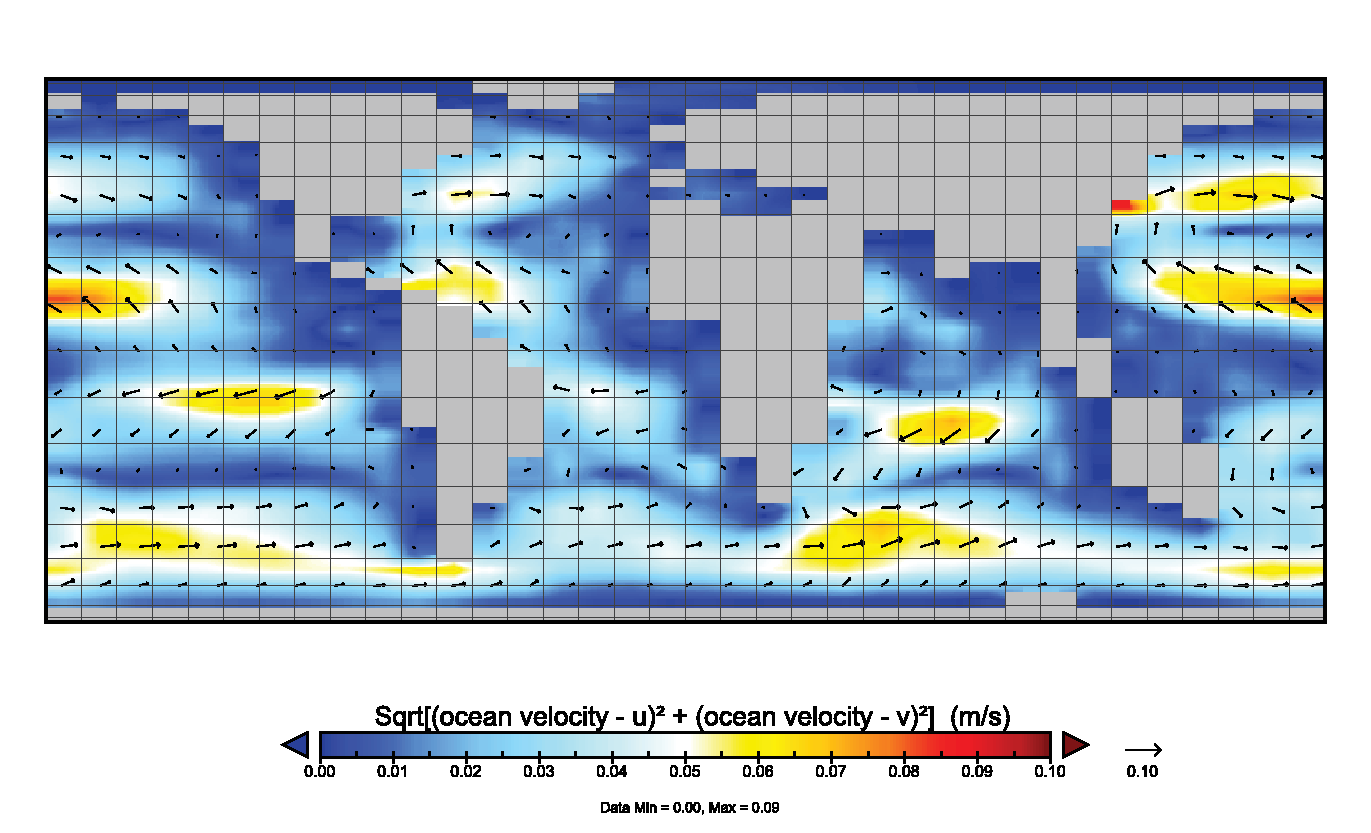
\includegraphics[scale=0.5]{cgenie_currents.eps}
\end{center}
\caption{Example (modern) ocean surface velocity (current) map.}
\label{fig:cgenie_currents}
\end{figure}

%---------------------------------------------------------------------------------------------------------------------------------
%---------------------------------------------------------------------------------------------------------------------------------

\subsection{MUTLAB plotting}

Several functions are provided for plotting \textit{BIOGEM} and \textit{SEDGEM} \textit{netCDF} output.
These can be found in the \texttt{cgenie} sub-directory: \texttt{\~{}/genie-matlab}.
The plotting functions and have on-line 'help', i.e., type:
\vspace{-10pt}\begin{verbatim}>> help functionname\end{verbatim}\vspace{-10pt}
where \texttt{functionname.m} is one of:

\begin{compactenum}
	\item \texttt{plot\_fields\_biogem\_2d.m} -- Plot a 2-D field from: \texttt{fields\_biogem\_2d.nc}.
		\item \texttt{plot\_fields\_biogem\_3d\_i.m} -- Plot a vertical-meridional (2-D) slice through the ocean (i.e., all cells have the same \texttt{i} (longitudinal) coordinate value) from: \texttt{fields\_biogem\_2d.nc}. Options are also provided for averaging longitudinally over a supplied mask, which may be the entire ocean and hence giving a global meridional cross-sectional mean, of a specific ocean basin, or may be a single cell 'wide' longtudinally and take a meandering path hence simulating an ocean transect. An option is provided to overlay ocean circulation streamfunctions.
		\item \texttt{plot\_fields\_biogem\_3d\_k.m} -- Plot a horizontal slice through the ocean. An option is provided for overlaying ocean circulation. Water column integrals can also be calculated and displayed.
		\item \texttt{plot\_fields\_sedgem\_2d.m} -- plot a 2-D field from: \texttt{fields\_sedgem\_2d.nc}.
\end{compactenum}
All 4 plotting functions can also overlay observed data and create difference (anomaly) maps -- either between different experiments, time-slices, or variables, or between model and data and provide summary statistics regarding the difference.

\subsubsection{Argument (parameter) list}

All 4 plotting functions share exactly the same format of parameters\footnote{Parameters can be in for form of strings, in which case they must be given as a series of characters enclosed in inverted commas \texttt{''}; as real numbers, e.g. \texttt{999.5} or \texttt{9.995E2}; or integers, e.g. \texttt{2}, \texttt{10}.}. passed in the argument list:
\texttt{functionname(PAR1,PAR2,PAR3, ... PARn)}
i.e. take a (long!) list of parameters.
\noindent These are:

\begin{compactitem}
\item \texttt{PPATH} -- is the relative pathway to the directory location of the experiments. For example, if all the individually-named experiment directories are located in a directory named \texttt{cgenie\_output} (as per how results are saved by default by the model), and this directory is located in the same directory as the MATLAB function is being run, parameter \texttt{PATH} takes the value: \texttt{'cgenie\_output'}.\footnote{Note that as a string value, the inverted commas are important.} If the experiment directory was located in the same directory as the MATLAB function, a null value must be passed, i.e., \texttt{''}.
\end{compactitem}
There are then a series of parameters for defining experiment, variable, and year, and whether difference (anomaly) maps are to be generated:
\begin{compactitem}
\item \texttt{PEXP1} -- is the name of the 1st (main) experiment.
\item \texttt{PEXP2} -- is the name of the 2nd (optional) experiment. If no second experiment is selected, then a null string value must be passed, i.e., \texttt{''}.
\item \texttt{PVAR1} -- is the name of the 1st (main) variable. If no valid variable value is given, a list of valid variable names will be printed out.\footnote{As a string, the value must be encased in inverted commas: \texttt{''}.}
\item \texttt{PVAR2} -- is the name of the 2nd (optional) variable. If no second variable is selected, then a null string value must be passed, i.e., \texttt{''}.
\item \texttt{PT1} -- is the value of the 1st (main) time-slice. If no valid variable value is given, a list of valid variable names will be printed out.\footnote{As \textit{sedgem} does not save multiple and/or time-specific data, a dummy value (anything) is entered here.}
\item \texttt{PT2} -- is the value of the 2nd (optional) time-slice. If no second time-slice is selected, then enter \texttt{-1}.\footnote{As \textit{sedgem} does not save multiple and/or time-specific data, a dummy value (anything) is entered here.}
\end{compactitem}
There are 2 parameters for plotting sub-sets of the 2D or 3D data (essential for 3D data which cannot be usefully visualized in raw form):
\begin{compactitem}
\item \texttt{PIK} -- varies in its interpretation and is discussed below.
\item \texttt{PMASK} -- is the name of an optional (2D) mask. A null string (\texttt{''}) must be passed if no mask is requested. The interpretation of this parameter differs slightly between functions (below).
\end{compactitem}
Next come options for plotting scale control:
\begin{compactitem}
\item \texttt{PCSCALE} -- is the scale factor for the plot. For example, to plot in micro molar (umol kg-1) units, enter; \texttt{1e-6}. The plot is auto-scaled if a value of zero (\texttt{0.0}) is entered.
\item \texttt{PCMIN} -- is the minimum scale value.
\item \texttt{PCMAX} -- is the maximum scale value.
\item \texttt{PCN} -- is the number of (contour) intervals between minimum and maximum scale values.
\end{compactitem}
Finally, there are 2 parameters for substituting an alternative title to the plot and for specifying discrete (observed) data to be plotted (and analyzed against model projections):
\begin{compactitem}
\item \texttt{PTIT} -- is the string for the alternative plot title. This parameter must be passed as a string, e.g., \texttt{'distribution of bottom-water phosphate concentrations'}. If an empty (i.e., \texttt{''}) value is passed to this parameter then a title is automatically generated.
\item \texttt{PDATA} -- is the filename containing the an overlay data set, which must be formatted as separated columns of: lon, lat, value. The full filename of this file must be give, including any extensions. This parameter must be passed as a string; leave blank, i.e., \texttt{''}, for no overlay data.
\end{compactitem}

The basic parameter list to all 4 plotting functions is hence:
\vspace{-10pt}\begin{verbatim}
functionname
(PPATH,PEXP1,PEXP2,PVAR1,PVAR2,PT1,PT2,PIK,PMASK,PCSCALE,PCMIN,PCMAX,PCN,PTIT,PDATA)
\end{verbatim}\vspace{-10pt}

Note that for \texttt{plot\_fields\_sedgem\_2d.m} several of the parameters are redundant but \textbf{must} be included (typically as zeros). This is in order to retain a common parameter list format between all the different plotting functions.

\subsubsection{Function specific interpretation of PIK and PMASK}

\texttt{PIK} and to some extent \texttt{PMASK} have quite different interpretations depending on the particular plotting functions:

\begin{compactenum}

\item \texttt{plot\_fields\_biogem\_2d.m}
\begin{compactitem}
\item \texttt{PIK} -- is the maximum depth (\texttt{k}) level that will be plotted, i.e. all depth levels deeper than \texttt{PIK} will be excluded. This is useful for plotting a variable only for the 'deep' ocean (rather than the ocean overlaying all ocean depths) for example. This value also provides an alternative way of creating a mask, and only values of \texttt{k} less than of equal to the passed value will be plotted.
\item \texttt{PMASK} -- is the name of an optional (2D) mask. A null string (\texttt{''}) must be passed if no mask is requested. (Shallow depths could also be excluded from the plot by means of a mask rather than setting \texttt{PIK}.)
\end{compactitem}

\item \texttt{plot\_fields\_biogem\_3d\_k.m}
\begin{compactitem}
\item \texttt{PIK} -- the depth (\texttt{k}) level to be plotted. Note that the levels are numbered from a maximum value designating the surface, to 1 for the deepest ocean level. Typically, maximum values for the number of ocean levels are \texttt{8} (e.g. \textit{Ridgwell et al.} [2007]) or \texttt{16} (e.g. \textit{Cao et al.} [2009]).
(\texttt{plot\_fields\_biogem\_3d\_i.m}) to be plotted. For \texttt{fields\_biogem\_2d.nc}, 
Zero values have special meanings here -- in \texttt{plot\_fields\_biogem\_3d\_k.m}, a zero will result in a water column inventory map being plotted.
\item \texttt{MASK} -- is the name of an optional (2D) mask. A null string (\texttt{''}) must be passed if no mask is requested.
\end{compactitem}

\item \texttt{plot\_fields\_biogem\_3d\_i.m}
\begin{compactitem}
\item \texttt{PIK} -- the longitude-depth (\texttt{i}) slice through the ocean to be plotted.
\item \texttt{MASK} -- is the name of an optional (2D) mask. A null string (\texttt{''}) must be passed if no mask is requested.
\\ For example: if the mask is of the entire ocean (\texttt{mask\_worbe2\_ALL.dat}), the result is a global meridional cross-sectional mean.
\\ If the mask is just of a single basin such as the Atlantic (\texttt{mask\_worjh2\_Atlantic.dat}), the result is the Atlantic meridional cross-sectional mean.
\\ Masks can also be constructed that are only a single cell 'wide' longtudinally, but which take a meandering path following an ocean transect\footnote{e.g., as in: \texttt{mask\_worjh2\_GEOSECS\_WATL.dat}}.
\\ The trivial usage would be to construct a mask consisting of a vertical line of \texttt{1}s -- the result is equivalent to setting an appropriate \texttt{i} value in \texttt{PIK}.
\end{compactitem}

\item \texttt{plot\_fields\_sedgem\_2d.m} is an exception as it does not (currently) use either parameter. \texttt{PIK} must be entered as \texttt{0} (any integer will do in fact), and \texttt{PMASK} as \texttt{''}.

\end{compactenum}

The mask itself (if \texttt{MASK} is set) is a 2-D array of model grid points (on the BIOGEM grid) in the form of a simple ASCII file. A value of '\texttt{1}' represents a vertical column of ocean cells to include, whereas a value '\texttt{0}' will exclude all cells in the water column at that particular grid point. Examples of masks can be found in the \texttt{genie-matlab} directory.
	
\subsubsection{Argument (parameter) list: Basic examples}

For example:
\\ {\small\texttt{plot\_fields\_sedgem\_2d('cgenie\_output','experiment\_1','','sed\_CaCO3','',0.0,0.0,0,'',\\1.0,0.0,100.0,20,'wt\% CaCO3','caco3.dat')}}
\\ plots plot the carbonate content of surface sediments, between 0 and 100 wt\% in 20 contour intervals, with an overlain observational dataset defined in the file \texttt{caco3.dat} and a specific title. The section '\texttt{,0.0,0.0,0,'',}' near the middle are the dummy variables (time-slice and alternative time-slice, i/k value, and mask) introduced for consistency in format with the other 3 plotting functions.

\subsubsection{Further refinements}

A number of additional options for exerting finer control over the plotting are provided as a block of parameters and (default) values in the m-file itself, in a section immediately after the commented help and change-log at the start of the m-file. Not all the options are relevant to all the plotting functions\footnote{See 'help' on a specific plotting function for details of the relevant options in the parameter block.}, but the full list (and then defaults in brackets \texttt{[]}) is as follows:

{\small \begin{compactitem}
\item \texttt{lon\_min = -180;         [-180]  STARTING LONGITUDE FOR X-AXIS}
\\ Sets the longitude of the left-hand edge of the plot.
\item \texttt{delta\_lon = 90;         [  90]  INCREMENT OF LONGITUDE ON X-AXIS}
\\ Sets the longitude tick increment.
\item \texttt{contour\_plot = 'n';     [ 'n']  OVERLAY CONTOL PLOT?}
\\ Overlay line contours on the color block plot?
\item \texttt{contour\_mod = 2;        [   2]  NUMBER OF COLOR INTERVALS PER CONTOR}
\\ Number of color graduations per line contour.
\item \texttt{contour\_mod\_label = 4;  [   4]  NUMBER OF LABELED CONTOURS PER CONTOUR}
\\ Number of color graduations per labeled line contour.
\item \texttt{contour\_label = 'y';    [ 'y']  LABEL CONTOURS?}
\\ Label the line contours (frequency of labeled contours set by \texttt{contour\_label}.
\item \texttt{contour\_noneg = 'n';    [ 'n']  RESTRICT DATA PLOTTED TO > 0.0?}
\\ Restrict the plotted values to non-negative? (Can be useful if slightly negative values exist as can occur during tracer transport associated with large concentration gradients.)
\item \texttt{plot\_log10 = 'n';       [ 'n']  PLOT LOG10 OF THE DATA}
\\ Plot data values as log10(value)?
\item \texttt{contour\_zero = 'y';     [ 'y']  PLOT ZERO CONTOUR}
\\ Plot the zero contour?
\item \texttt{colorbar\_old = 'n';     [ 'n']  PLOT 'OLD' COLORBAR}
\\ Plot old style colorbar.
\item \texttt{data\_offset = 0.0;      [ 0.0]  data offset (273.15 for K -> C)}
\\ Introduce a data offset? This is useful for example for converting K to degrees C (removing the K value of 0 degrees C).
\item \texttt{data\_ij = 'n';          [ 'n']  DATA as (i,j)?}
\\ Overlay data in the form of (i,j) locations rather than longitude,latitude?
\item \texttt{data\_ijk = 'n';          [ 'n']  DATA as (i,j,k)?}
\\ Overlay data in the form of (i,j,k) locations rather than longitude, latitude, depth?
\item \texttt{data\_ij\_mean = 'n';     [ 'n']  average DATA by cell?}
\\ Average overlay data per \textit{c}GENIE grid cell rather than plotting raw locations.
\item \texttt{data\_ijk\_mean = 'n';     [ 'n']  average DATA by cell?}
\\ Average overlay data per \textit{c}GENIE grid cell rather than plotting raw locations.
\item \texttt{data\_size = 25.0;       [25.0]  SIZE OF OVERLAY DATA POINTS}
\\ Size of the overlay data points.
\item \texttt{data\_anomoly = 'n';     [ 'n']  PLOT AS MODEL-DATA ANOMOLY ONLY?}
\\ Plot data locations with the model-data anomaly rather than data value?
\item \texttt{data\_only = 'n';        [ 'n']  PLOT ONLY DATA (no model values)?}
\\ Plot only the overlay data locations (and not any model data)?
\item \texttt{data\_site = 'n';        [ 'n']  PLOT DATA AS SITES (no data values)?}
\\ Plot labeled site locations (no data value fill).
\item \texttt{plot\_land = 'n';        [ 'n']  PLOT DATA OVER LAND?}
\\ Plot data locations lying over land on the \textit{c}GENIE grid (rather than screen out)?
\item \texttt{data\_uv = 'n';          [ 'n']  overlay (u,v) velocity data?}
\\ Overlay ocean current fields.
\item \texttt{data\_uv\_scale = 1.0;    [ 1.0]  scaling factor for vector length}
\\ Scaling factor for velocity vectors.
\item \texttt{plot\_opsi = '';         [  '']  PLOT OVERTURNING STREAMFUNCTION (basin)?}
\\ Plot overturning streamfunction overlay?
\item \texttt{plot\_opsi\_min = -15;    [ -15]; plot\_opsi\_max = +15;    [ +15]; 
plot\_opsi\_dminor = 1;   [   1]; plot\_opsi\_dmajor = 5;   [   5] }
\\ Controls on min, max and (major and minor) contor intervals.
\item \texttt{dscrsz = 0.60;          [0.60]  FRACTIONAL FIGURE WINDOW SIZE}
\\ Adjustment factor of the fractional size (compared to the screen) of the figure window.
\end{compactitem}}

\subsubsection{Further refinements: Examples}

Examples: 
\begin{compactenum}
\item To plot the positions (and labels) of data locations:
\\ {\small \texttt{plot\_fields\_biogem\_3d\_k('cgenie\_output','120926.SPIN','',49999.5,-1,'ocn\_temp','','',\\16,1.0,10.0,40.0,30,'','sites.dat')}}
\\ where the experiment name is \texttt{120926.SPIN}, the mapped variable is \texttt{ocn\_temp} (although no model field need be plotted -- set by an option in the plotting function itself, and the file of data locations is \texttt{sites.dat}.
\end{compactenum}

\begin{figure}[ht]
\begin{center}
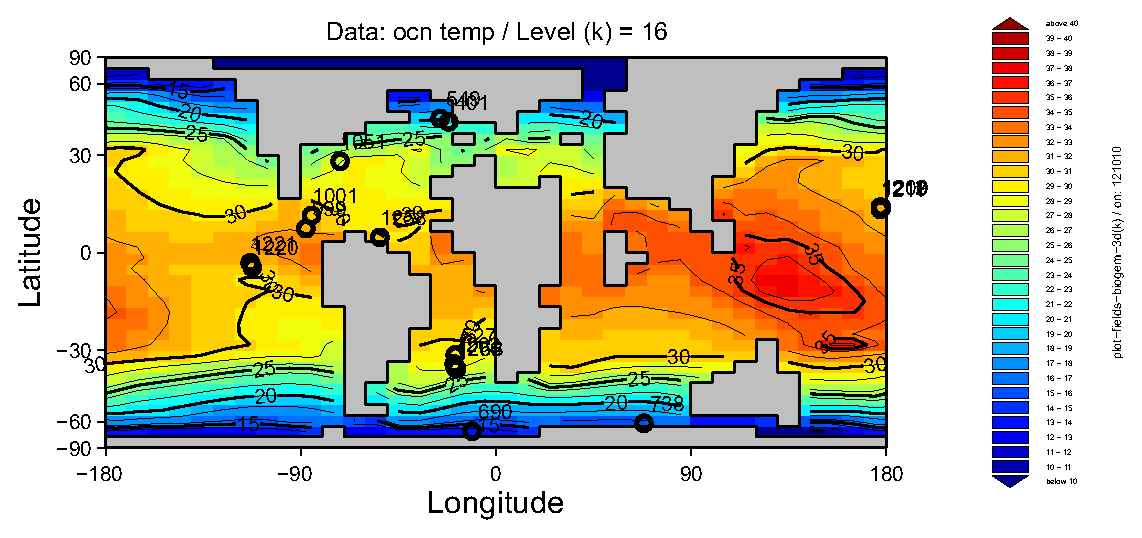
\includegraphics[scale=0.75]{cgenie_datalocations.eps}
\end{center}
\caption{Paleocene-Eocene deep-sea sediment drill locations together with a contour-overlain map of surface temperature.}
\label{fig:cgenie_datalocations}
\end{figure}

%=================================================================================================================================
%=== APPENDICES ==================================================================================================================
%=================================================================================================================================

\appendix

%---------------------------------------------------------------------------------------------------------------------------------
%--- Appendix A: Quick-start guide -----------------------------------------------------------------------------------------------
%---------------------------------------------------------------------------------------------------------------------------------

\newpage
\section{Quick-start guide}\label{Appendix A}

\begin{compactenum}
\item	To get a (read-only) copy of the current (development) branch of \textit{c}GENIE source code:
\\ From your home directory (or elsewhere, but several path variables will have to be edited -- see below), type:
\vspace{-5pt}\begin{verbatim}
svn co https://svn.ggy.bris.ac.uk/subversion/genie/tags/cgenie.muffin-0.4
--username=genie-user cgenie.muffin
\end{verbatim}\vspace{-5pt}
NOTE: All this must be typed continuously on ONE LINE, with a S P A C E before `\texttt{--username}', and before `\texttt{cgenie}'.
You will be asked for a password -- it is \texttt{g3n1e-user}.

\item	If you are installing on your own machine (i.e. not a Bristol (c)genie friendly cluster) you are likely to have to set a couple of environment variables. The compiler name, netCDF library name, and netCDF path, are specified in the file \texttt{user.mak} (\texttt{genie-main} directory). If the \textit{c}genie code tree (cgenie.muffin) and output directory (cgenie\_output) are installed anywhere other than in your account HOME directory, paths specifying this will have to be edited in: \texttt{user.mak} and \texttt{user.sh} (\texttt{genie-main} directory).
		
\item	Change directory to \texttt{cgenie.muffin/genie-main} and type:
\vspace{-5pt}\begin{verbatim}
make testbiogem
\end{verbatim}\vspace{-5pt}
This compiles a carbon cycle enabled configuration of \textit{c}GENIE and runs a short test, comparing the results against those of a pre-run experiment (also downloaded alongside the model source code). It serves to check that you have the software environment correctly configured. If you are unsuccessful here ... double-check the software and directory environment settings in \texttt{user.mak} or \texttt{user.sh}.

\item	At this point, the science modules are currently compiled in a grid and/or number of tracers configuration that is unlikely to be what you want for running experiments. Clean up all the compiled \textit{c}GENIE modules, ready for re-compiling from the source code, by:
\vspace{-5pt}\begin{verbatim}
make cleanall
\end{verbatim}\vspace{-5pt}
  
\end{compactenum}

That is it as far as basic installation goes. Except to read the \textit{c}GENIE \texttt{User\_manual} ;)
\\ (Also see: \textit{c}GENIE \texttt{README} and \textit{c}GENIE \texttt{HOWTO} documents.)

%---------------------------------------------------------------------------------------------------------------------------------
%--- Appendix B: Available GENIE modules -----------------------------------------------------------------------------------------
%---------------------------------------------------------------------------------------------------------------------------------

\newpage
\section{Available GENIE modules}\label{Appendix B}

\begin{figure}[h]
%\resizebox{\columnwidth}{!}{
%\includegraphics*[bb=0 0 100 100]{genie_modules.eps}}
\includegraphics*{genie_modules.eps}
\caption{Table summarizing the different GENIE modules.}
\label{fig:genie_modules}
\end{figure}

%---------------------------------------------------------------------------------------------------------------------------------
%--- Appendix C: GENIE directory structure ---------------------------------------------------------------------------------------
%---------------------------------------------------------------------------------------------------------------------------------

\newpage
\section{cGENIE directory structure}\label{Appendix C}

This section describes the directories and files pertinent to configuring and running biogeochemistry experiments in cGENIE.

\begin{figure}[h]
\includegraphics*{genie_filetree.eps}
\caption{Schematic of the cGENIE file-tree. Note that only the sub-directory structure for the \texttt{genie-biogem} module is shown expanded; near-identical sub-structures are present in all the science modules. The dark gray shaded parts of the directory tree are not part of the official GENIE release, but instead required when using the \texttt{old\_rungenie.sh} script. The light gray branch is required only when submitting cluster jobs exactly as described in this document. 
The directory in which the genie code tree is installed is assumed to be your home directory and is designated by \texttt{\~{}}.}
\label{fig:genie_filetree}
\end{figure}

The details of the directory contents are as follows.

\begin{compactitem}

	\item \texttt{\~{}/cgenie/genie-atchem/data/input}
	\\Input data files for the atmospheric chemistry module ATCHEM. Currently there are no data files that are required to be present here.
	
	\item	\texttt{\~{}/cgenie/genie-atchem/src/fortran}
	\\Source code for the atmospheric chemistry module ATCHEM:
	\begin{compactitem}
		\item \texttt{atchem.f90} -- Updating of atmospheric composition; re-start file saving.
		\item \texttt{atchem\_box.f90} -- [currently just an empty template module - will hold atmospheric 'chemistry' subroutines]
		\item \texttt{atchem\_data.f90} -- Load re-start; initialize atmospheric grid and tracers; read in namelist settings.
		\item \texttt{atchem\_lib.f90} -- Parameter and array definitions having ATCHEM module scope; set namelist definitions.
		\item \texttt{cpl\_comp\_atmocn.f90} -- Set surface-atmosphere trace-gas interface composition.
		\item \texttt{cpl\_flux\_ocnatm.f90} -- Integrate net trace-gas flux to atmosphere from surface.
		\item \texttt{end\_atchem.f90} -- [currently does not 'do' anything except print-to-screen]
		\item \texttt{initialise\_atchem.f90} -- Initialize ATCHEM; read in name-list settings.
		\item \texttt{makefile} -- Errr, the makefile ... :o)
	\end{compactitem}
	
	\item \texttt{\~{}/cgenie/genie-biogem/data/input}
	\\Input data files for the ocean biogeochemistry module BIOGEM. This is the location searched for input data files if the default input directory namelist setting is used, which is set by the namelist parameter: \texttt{bg\_par\_indir\_name}. In addition to any files added locally (e.g., for specific model runs) the SVN server holds the following files:
	\begin{compactitem}
		\item Default\footnote{These are configured for no selected forcings.} configuration of tracer forcing of BIOGEM:
		\begin{compactitem}
			\item \texttt{configure\_forcings\_atm.dat} -- Selection and configuration of forcing of atmospheric (gas) tracers.
			\item \texttt{configure\_forcings\_ocn.dat} -- Selection and configuration of forcing of ocean (dissolved) tracers.
			\item \texttt{configure\_forcings\_sed.dat} -- Selection and configuration of forcing of sediment (particulate matter) tracers.
		\end{compactitem}
		\item Configuration files for use in the BIOGEM test (\texttt{\$ make testbiogem}):
		\begin{compactitem}
			\item \texttt{genie\_eb\_go\_gs\_ac\_bg\_test\_save\_sig.dat} -- Specification of the times of time-series data saving.
			\item \texttt{genie\_eb\_go\_gs\_ac\_bg\_test\_save\_timeslice.dat} -- Specification of the times of time-slice data saving.
			\item \texttt{genie\_eb\_go\_gs\_ac\_bg\_test\_windspeed.dat} -- Prescribed wind field for calculating air-sea gas exchange.
		\end{compactitem}
		\item Various illustrative (template) time-series data saving specification files:
		\begin{compactitem}
			\item \texttt{save\_sig\_historical.dat} -- Time-series saves specified to cover 1765.5 to 2000.5 at 1.0 year intervals, with 0.5 to 1000.5 following \texttt{save\_sig\_log10.dat} (below).
			\item \texttt{save\_sig\_log10.dat} -- Time-series saves specified at intervals of 1.0 years up until 10.5 years, then 10.0 years until 100.5 years, etc etc.
			\item \texttt{save\_sig\_log10\_25kend.dat} -- As above, but terminating at 25000.5 (i.e., the mid-point of the year 25000).
			\item \texttt{save\_sig\_log10\_50kend.dat} -- As above, but terminating at 50000.5 (i.e., the mid-point of the year 25000).
		\end{compactitem}
		\item Various illustrative (template) time-slice data saving specification files:
		\begin{compactitem}
		\item \texttt{save\_timeslice\_historical.dat} -- Time-slice saves specified with mid-points at: 1765.5, 1994.5, 2000.5.
			\item \texttt{save\_timeslice\_log10.dat} -- Time-slice saves specified with mid-points at: 0.5, 10.5, 100.5, 1000.5, etc etc.
			\item \texttt{save\_timeslice\_log10\_25kend.dat} -- As above, but terminating at 25000.5.
			\item \texttt{save\_timeslice\_log10\_50kend.dat} -- As above, but terminating at 50000.5.
		\end{compactitem}
	\item Modern observed annual mean wind-speed for use as an air-sea gas exchange boundary condition in BIOGEM\footnote{The alternative is to estimate wind-speed and hence calculate air-sea gas exchange from the wind-stress field applied to the GOLDSTEIN ocean circulation model. The wind-stress based reconstruction can be chosen by setting: \texttt{bg\_ctrl\_force\_windspeed=.false.}}:
		\begin{compactitem}
			\item \texttt{windspeed.dat}
		\end{compactitem}
	\end{compactitem}
	
	\item \texttt{\~{}/cgenie/genie-biogem/src/fortran}
	\\Source code for the ocean biogeochemistry module BIOGEM:
	\begin{compactitem}
		\item \texttt{biogem.f90} - Primary ocean biogeochemical cycling subroutine/loop; saving of time-series and time-slice data; re-start file saving.
		\item \texttt{biogem\_box.f90} -- Ocean biogeochemical cycling calculations; time-dependent forcing updating; tracer 'auditing' calculations.
		\item \texttt{biogem\_data.f90} -- Load re-start; initialize ocean grid and tracers; ASCII time-series data saving; ASCII time-slice data saving; read in name-list\footnote{Would more logically live in \texttt{initialise\_atchem.f90} ...}.
		\item \texttt{biogem\_data\_netCDF.f90} -- netCDF format time-slice data saving.
		\item \texttt{biogem\_lib.f90} -- Parameter and array definitions having biogem module scope; set namelist definitions
		\item \texttt{end\_biogem.f90} -- Final auditing and reporting.
		\item \texttt{initialise\_biogem.f90} -- Initialize BIOGEM; read in name-list settings.
		\item \texttt{makefile} -- Errr, the makefile ... :o)
	\end{compactitem}
	
	\item \texttt{\~{}/cgenie/genie-main}
	[see: GENIE wiki pages]
	
	\item \texttt{\~{}/cgenie/genie-main/configs}
	[see: ...]
	
	\item \texttt{\~{}/cgenie/genie-main/data/input}
	\\Input data files required by the cmngem module defining the tracers in the atmosphere, ocean, and sediments and the relationships between the different tracers:
	\begin{compactitem}
		\item \texttt{tracer\_define.atm}
		\item \texttt{tracer\_define.ocn}
		\item \texttt{tracer\_define.sed}
	\end{compactitem}
	The contents of these files must not be altered (nor the files moved, unless there is a very good reason to do so ...).
	\\Since there never will be a 'very good reason' ... \textbf{HANDS OFF}.
	
	\item \texttt{\~{}/cgenie/genie-main/src/fortran/cmngem}
	\\Source code for the geochemistry library modules -- common routines, constants, and parameters that need to be accessed by all biogeochemistry modules (i.e., ATCHEM, BIOGEM, SEDGEM, and ROKGEM). The source code files are:
	\begin{compactitem}
		\item \texttt{gem\_carbchem.f90} -- Definition and solution of aqueous carbonate chemistry; routines for solving isotopic fractionation; routines for estimating DIC and ALK given other parameters.
		\item \texttt{gem\_cmn.f90} -- Parameter and constant definitions.
		\item \texttt{gem\_data.f90} -- Read in namelist parameters.
		\item \texttt{gem\_netcdf.f90} -- Low-level netCDF file I/O routines.
		\item \texttt{gem\_util.f90} -- Miscellaneous routines, such as for reading and writing ASCII file formats, converting between isotopic notations, numerical solution and multi-dimensional linear interpolation, initialization of tracers and inter-tracer relationships
		\item initialise\_gem.f90 -- Tracer property and relationship definition.
	\end{compactitem}

	\item \texttt{\~{}/cgenie/genie-matlab}
	\\MUTLAB scripts for plotting fields from the 2-D and 3-D BIOGEM and SEDGEM netCDF results files, plus related plotting configuration files.
	
	\item \texttt{\~{}/cgenie/genie-rokgem/data/input}
	\\ ...
	
	\item \texttt{\~{}/cgenie/genie-rokgem/src/fortran}
	\\ ...
	
	\item \texttt{\~{}/cgenie/genie-sedgem/data/input}
	\\Input data files for the (deep-sea) sediment biogeochemistry module SEDGEM. This is the location searched for input data files if the default input directory namelist setting is used, whihc is set by the namelist parameter: \texttt{sg\_par\_indir\_name}. In addition to any files added locally (e.g., for specific model runs) the SVN server holds the following files:
	\begin{compactitem}
		\item Masks which specify the sediment grid locations at which sediment cores are generated:
		\begin{compactitem}
			\item \texttt{sedgem\_save\_mask.36x36} -- ... .
			\item \texttt{sedgem\_save\_mask.72x72} -- ... .
		\end{compactitem}
		\item Bioturbational mixing profile:
		\begin{compactitem}
			\item \texttt{sedgem\_sed\_mix\_k.dat} -- ... .
		\end{compactitem}
		\item Sediment grid topography (bathymetry):
		\begin{compactitem}
			\item \texttt{sedgem\_topo\_D.36x36} -- ... .
			\item \texttt{sedgem\_topo\_D.72x72} -- ... .
		\end{compactitem}
	\end{compactitem}
	
	\item \texttt{\~{}/cgenie/genie-sedgem/src/fortran}
	\\Source code for the ocean sediments biogeochemistry module SEDGEM:
	\begin{compactitem}
		\item \texttt{cpl\_comp\_sedocn.f90} -- ... .
		\item \texttt{cpl\_flux\_sedocn.f90} -- ... .
		\item \texttt{end\_sedgem.f90} -- Final auditing and reporting.
		\item \texttt{initialise\_sedgem.f90} -- Initialize SEDGEM; read in name-list settings.
		\item \texttt{sedgem.f90} -- Primary ocean biogeochemical cycling subroutine/loop; saving of time-series and time-slice data; re-start file saving.
		\item \texttt{sedgem\_box.f90} -- Ocean biogeochemical cycling calculations; time-dependent forcing updating; tracer 'auditing' calculations.
		\item \texttt{sedgem\_box\_archer1991\_sedflx.f90} -- ... .
		\item \texttt{sedgem\_box\_ridgwell2001\_sedflx.f90} -- ... .
		\item \texttt{sedgem\_data.f90} -- Load re-start; initialize ocean grid and tracers; ASCII time-series data saving; ASCII time-slice data saving; read in name-list.
		\item \texttt{sedgem\_data\_netCDF.f90} -- netCDF format time-slice data saving.
		\item \texttt{sedgem\_lib.f90} -- Parameter and array definitions having SEDGEM module scope; set namelist definitions.
		\item \texttt{sedgem\_nnutils.f90} -- Neural network utilities.
		\item \texttt{makefile} -- Errr, the makefile ... :o)
	\end{compactitem}
	
	\item \texttt{\~{}/cgenie\_archive} -- This directory \texttt{IS NOT} created automatically for you and is where the \texttt{old\_rungenie.sh} run script will attempt to put archived results.
	
	\item \texttt{\~{}/genie\_forcings} -- This directory \texttt{IS NOT} created automatically for you.
	
	\item \texttt{\~{}/cgenie\_log} -- The location where standard output and error streams are directed into a file. This directory \texttt{IS NOT} created automatically for you.
	
	\item \texttt{\~{}/cgenie\_output} -- The default directory where the results will be sent. This directory \texttt{IS} created automatically for you.
	
	\item \texttt{\~{}/genie\_userconfigs}
	
\end{compactitem}

%---------------------------------------------------------------------------------------------------------------------------------
%--- Appendix D: namelist parameter definitions and defaults ---------------------------------------------------------------------
%---------------------------------------------------------------------------------------------------------------------------------

XXX CONTINUE XXX

\newpage
\section{Namelist parameter definitions and defaults}\label{Appendix D}

Parameters in the model are controlled via \textit{namelists} -- lists of parameter names whose values are passed into GENIE when it initializes. The default namelist parameter values are listed in a set of Tables, which can be downloaded from \textit{mygenie.seao2.org}. These are the values and settings that GENIE will use if not told otherwise. 

To effect a change in parameter value, the parameter name is simply assigned the new value, either in the \textit{base config} used, i.e. one of the \texttt{.config} files in:
\vspace{-5.5pt}\begin{verbatim}~/genie/genie-main/configs\end{verbatim}\vspace{-5.5pt}
Or, more typically, when using the \texttt{old\_rungenie.sh} model job configuration and submission script: by appending the new namelist assignment(s) to the \textit{user config} file defining the experiment in:
\vspace{-5.5pt}\begin{verbatim}~/genie_userconfigs\end{verbatim}\vspace{-5.5pt}
Either way, the (re-)assignment generally takes the form:
\vspace{-5.5pt}\begin{verbatim}namelist = value\end{verbatim}\vspace{-5.5pt}
Where the value is a string, the syntax is:
\vspace{-5.5pt}\begin{verbatim}namelist = 'string'\end{verbatim}\vspace{-5.5pt}
The syntax for logical flag (e.g., 'true') assignments is:
\vspace{-5.5pt}\begin{verbatim}namelist = .true.\end{verbatim}\vspace{-5.5pt}

For selecting (or de-selecting) tracers, the syntax is:
\vspace{-5.5pt}\begin{verbatim}gm_atm_select_nn = .true.\end{verbatim}\vspace{-5.5pt}
for an atmospheric tracer (gas). \texttt{nn} is the integer index of the tracer as detailed in the Tables. For ocean and sediment (particulate) tracers, the namelist names take the same form except with \texttt{ocn} or \texttt{sed} in the namelist parameter name.

If the number of selected tracers in the ocean is changed, so to must the value of \texttt{GOLDSTEINNTRACS}, which sets the ocean array dimension and the number of tracers that must be advected, convected, and diffused. The value of \texttt{GOLDSTEINNTRACS} must be equal to the number of selected ocean tracers (i.e., the number of \texttt{gm\_ocn\_select\_nn} that are \texttt{.true.}) \textit{including} temperature (T) and salinity (S). The default value is 2 (just T and S, giving climate-only simulation capabilities), but this value is adjusted in the \texttt{.config} files. Any further deviation from the ocean tracer selection requires a new value to be assigned in the \textit{user config}.

\noindent For example, for 16 selected ocean tracers (including temperature and salinity), add the line:
\vspace{-5.5pt}\begin{verbatim}GOLDSTEINNTRACSOPTS = '$(DEFINE)GOLDSTEINNTRACS=16'\end{verbatim}\vspace{-5.5pt}
to the end of the \textit{user config} file

For setting initial values of tracers, the syntax is:
\vspace{-5.5pt}\begin{verbatim}gm_atm_init_nn = 278.0E-6\end{verbatim}\vspace{-5.5pt}
in the case of an atmospheric (gaseous) tracer. Again, \texttt{nn} is the index of the tracer. Ocean tracers are initialized similarly\footnote{There is no user-configurable initialization of deep-sea sediment composition (in SEDGEM).}. The units of the tracer initialization parameters are given in the summary Tables.

%---------------------------------------------------------------------------------------------------------------------------------
%--- Appendix E: The runcgenie.sh script --------------------------------------------------------------------------------------
%---------------------------------------------------------------------------------------------------------------------------------

\newpage
\section{The \texttt{runcgenie.sh} script}\label{Appendix E}

%---------------------------------------------------------------------------------------------------------------------------------
%---------------------------------------------------------------------------------------------------------------------------------

\subsection{Overview}
The overall strategy for the \texttt{runcgenie.sh} methodology of running \textit{c}GENIE is as follows:

\begin{compactenum}

	\item Copy a \texttt{.config} file\footnote{As outlined earlier, the specification of particular flavors (unique combinations of science modules) are contained in \texttt{.config} files with names of the form \texttt{genie\_aa\_oo\_ss\_xxxx.config}. For instance, a configuration + parameter calibration of the 16-level version of the GOLDSTEIN ocean model together with ocean biogeochemistry, is defined in \texttt{genie\_eb\_go\_gs\_ac\_bg\_itfclsd\_16l\_JH.config}} defining the required flavor of GENIE plus configuration and calibration of the climatology from \texttt{\~{}/genie/genie-main/configs}.
	
	\item Append a series of \textit{namelist} parameter values changes specific to a particular model experiment, particularly those involving the biogeochemistry and carbon cycling such as the specification of a CO2 emissions forcing \footnote{The details of any biogeochemical forcings are stored in a directory specified by the value of the namelist parameter \texttt{bg\_par\_fordir\_name}.} or selection of feedbacks (e.g. CO2-and-climate, CO2-and-calcification).
	\\These namelist parameter alternations (compared to the defaults) are provided in the form of a 'patch' file.
	\\The altered configuration details are added (patched) to create a fine-tuned configuration \texttt{*.config} file with a name unique to the model experiment.
	\\For example\footnote{Refer to the tutorial for a detailed description of this particular model experiment.}, taking a basic science module flavor and configuration:
	\\\texttt{genie\_eb\_go\_gs\_ac\_bg.config}
	\\and modifying it according to the biogeochem experiment defined by:
	\\\texttt{\~{}/genie\_userconfigs/worbe2\_preindustrial\_1}
	\\results in the creation of a new configuration file:
	\\\texttt{genie\_eb\_go\_gs\_ac\_bg.worbe2\_preindustrial\_1.config}
	\\The new configuration file will contain additional settings such as:
	\begin{compactitem}
		\item The number of time-steps in the model in order to exactly achieve your requested run length
		\item Whether a re-start file is to be used or not, and if so, where the re-start files are located.
		\item The location of parameter files required by the various science modules.
	\end{compactitem}
	
	\item Finally, the working directory is changed to:
	\\\texttt{\~{}/genie/genie-main}
	\\and the model is automatically invoked in the 'usual way', i.e.:
	\begin{verbatim}$ ./genie_example.job -f 
	configs/genie_eb_go_gs_ac_bg.worbe2_preindustrial_1.config\end{verbatim}
	\textbf{BUT NOTE} that this is to illustrate what the \texttt{rungenie.sh} script does automatically for you and \texttt{DOES NOT} mean that you should necessarily enter in the \texttt{./genie\_example.job -f} command by hand (unless you have completely configured an experiment manually).
	
\end{compactenum}

%---------------------------------------------------------------------------------------------------------------------------------
%---------------------------------------------------------------------------------------------------------------------------------

\subsection{technical details}

In glorious and wonderful and completely tedious detail, \texttt{old\_rungenie.sh} actually does the following: 

\begin{compactenum}

	\item ACCEPT PASSED PARAMETERS
	\\Check that the required parameters (4) have been passed. Set local variables derived from passed parameters.
	
	\item SET LOCAL FILE AND DIRECTORY NAMES
	
	\item CREATE EXPERIMENT CONFIGURATION FILE
	\\Make a copy of the specified template configuration file (passed parameter \#1). Give the configuration file a unique filename by appending the model run ID (passed parameter \#3).
	
	\item SET MODEL TIME-STEPPING
	\\Set up the time-stepping control of model output, data saving, and experiment run length:
	\begin{compactitem}
		\item (a) Set run length in BIOGEM:
		\\ \texttt{bg\_par\_misc\_t\_start} is the start year, which is assumed to be zero by default.
		\\ \texttt{bg\_par\_misc\_t\_runtime} is the run length (years) -- its value is taken from passed parameter \#4.
 		\item (b) Based on the run length, a consistent overall GENIE run length in terms of the number of internal time-steps is set:
		\\\texttt{ma\_koverall\_total}, the overall number of internal time-steps in the model, is calculated based on the run length and length of each internal time-step.
		\\The length of each time-step is determined by the value of \texttt{ma\_genie\_timestep} (in seconds), and is defined in the \texttt{.config} file by:
		\\\texttt{ma\_genie\_timestep = 365.25*24.0/500 * 3600.0},
		\\i.e.,
		\\ \texttt{ma\_genie\_timestep=63115.2}
		\\giving 500 time-steps per year\footnote{For GENIE-1 flavors; a different time-step is used for GENIE-2 flavors.}.
		\\Note that also in \texttt{.config} file: \texttt{ma\_ksic\_loop=5} sets the updating of sea-ice to occur every 5 GENIE time-steps, and \texttt{ma\_kocn\_loop=5} set the updating of ocean circulation to occur every 5 GENIE time-steps.
		\\The \texttt{runtime\_defaults.sh} value of \texttt{ma\_katm\_loop=1} is unchanged, meaning that the atmosphere (the EMBM in this case) is updated each and every GENIE time-step.
		\\Finally, \texttt{ma\_dt\_write} sets a default interval of output (in multiples of the GENIE time-step), and is set equal to the total number of time-steps (\texttt{ma\_genie\_timestep}) to give output writing at the end of the experiment only.
		\item (c) Set the climate model components' restart saving frequency (iwstp):
		\\\texttt{ea\_4}, \texttt{go\_4}, and \texttt{gs\_4} set the frequency of restart saving (multiples of the GENIE time-step). These are set equal to \texttt{ma\_genie\_timestep} to give re-start saving only at the end of the run.
		\item (d) Set climate model components 'health check' frequency (npstp):
		\\\texttt{ea\_3}, \texttt{go\_3}, and \texttt{gs\_3} set the frequency of 'health check' diagnostics reporting.
		\\These are set equal to \texttt{ma\_genie\_timestep+1}, effectively disabling this feature.
		\item (e) Set climate model components 'time series' frequency (itstp):
		\\\texttt{ea\_5}, \texttt{go\_5}, and \texttt{gs\_5} set the frequeny of 'integral diagnostics' reporting.
		\\These are set equal to \texttt{ma\_genie\_timestep+1}, effectively disabling this feature.
		\item (f) Set climate model components 'average' frequency (ianav):
		\\\texttt{ea\_6}, \texttt{go\_6}, and \texttt{gs\_6} set the 'output averaging' interval.
		\\These are set equal to \texttt{ma\_genie\_timestep+1}, effectively disabling this feature.
		\item (g) Set ROKGEM terrestrial weathering model component reporting frequency:
		\\The value of \texttt{rg\_par\_screen\_output} is set equal to \texttt{ma\_genie\_timestep+1}, effectively disabling this feature.
	\end{compactitem}
	
	\item SET CLIMATE MODEL RE-START FILE DETAILS
	\begin{compactitem}
		\item (a) Set netCDF restart saving flag:
		\\The \texttt{'y'}/\texttt{'n'} value of \texttt{ea\_31}, \texttt{go\_19}, and \texttt{gs\_14} determine whether a netCDF format restart file is to be saved. These are set to \texttt{'n'}.
		\item (b) Set ASCII restart output flag:
		\\The \texttt{'y'}/\texttt{'n'} value of \texttt{ea\_32}, \texttt{go\_20}, and \texttt{gs\_15} determine whether an ASCII format restart file is to be saved.
		\item (c) Set ASCII 'restart number':
		\\\texttt{ea\_29}, \texttt{go\_17}, and \texttt{gs\_12} contain strings used to form the ASCII restart file names.
		\\The string is appented by \texttt{.\textit{n}}, where \texttt{\textit{n}} is an integer. The value of \texttt{\textit{n}} is incremented at each new re-start save. However, because the frequency of re-start saving has been configured to create only a single restart save at the end of the run, the extension of the restart file will always be \texttt{.1} when using \texttt{rungenie.sh} (unmodified).
	\end{compactitem}
	
	\item CONFIGURE USE OF RESTART
	\\Configure GENIE to use a restart (the alternative being to start from 'cold').
	\\Restart namelist items are set according to the presence or absence of the 5th passed parameter (restart experiment name).  If the 5th parameter is present when \texttt{rungenie.sh} is invoked, the following action is taken:
	\begin{compactitem}
		\item  (a) Check that the restart experiment (directory) exists. Generate an error message and exit if not.
		\item  (b) Set the climate model components to use a restart, namelist items:
		\\\texttt{ea\_7}, \texttt{go\_7}, \texttt{gs\_7}
		\\The syntax is \texttt{'c'} for a continuing run (i.e., using a restart), and \texttt{'n'} for new (from cold).
		\item (c) Set the biogeochemistry model components to use a restart, namelist items:
		\\\texttt{ac\_ctrl\_continuing}, \texttt{bg\_ctrl\_continuing}, \texttt{sg\_ctrl\_continuing}, (\texttt{rk\_ctrl\_continuing})
		\\The syntax is LOGICAL (\texttt{.true.} or \texttt{.false.}, or \texttt{t} or \texttt{f})
		\item (d) Set whether a netCDF restart is used for the climate model components:
		\\\texttt{ea\_30}, \texttt{go\_18}, \texttt{gs\_13}
		\\The syntax is \texttt{'n'} for no netCDF restart file format (instead it will be ASCII).
		\item (e) Set the climate model ASCII restart file name namelist values:
		\\\texttt{ea\_35}, \texttt{go\_23}, \texttt{gs\_18}.
		\\The name in each case is \texttt{'rst.1'} (\texttt{rst} being the default saved restart filename, and \texttt{.1} indicating the first saved restart (see above).
		\item (f) Set re-start location (given by optional parameter \#5).
		\\ The location of the re-start file for each module is given by a namelist parameter\footnote{A string describing the full path + filename - see page \pageref{Appendix D}.}: \texttt{xx\_rstdir\_name} in the case of the climate model modules and where \texttt{xx} is the module abbreviation (\texttt{ea}, \texttt{go}, \texttt{gs}), and \texttt{yy\_par\_rstdir\_name} in the case of the biogeochemical model modules, with \texttt{yy} being the module abbreviation (\texttt{ac}, \texttt{bg}, \texttt{sg}, \texttt{rg}).
	\end{compactitem}
	If restarts are not to be used, then:
	\\\texttt{ea\_7}, \texttt{go\_7}, \texttt{gs\_7} are all set to \texttt{'n'}, and
	\\\texttt{ac\_ctrl\_continuing}, \texttt{bg\_ctrl\_continuing}, \texttt{sg\_ctrl\_continuing}, \texttt{rk\_ctrl\_continuing} are all set to \texttt{.false.}.
	
	\item APPEND EXPERIMENT SPECIFIC NAMELIST CHANGES
	\\Append the contents of the user configuration file specified by the run ID (passed parameter \#3) and its directory location (passed parameter \#2) to the basic flavor and configuration file (parameter \#1).
	\\But first ... in case one has a Windoz user infestation ... the namelist file is conditioned to avoid possibility of carriage return/line-feed screw-ups\footnote{This step can be omitted (commented out/deleted) in the event that no Windoz users are involved}.
	\item GO!
	\\Run the model! Change directory and from \texttt{\~{}/genie/genie-main}, invoke:
	\vspace{-5.5pt}\begin{verbatim}./genie_example.job -f 
	configs/genie_eb_go_gs_ac_bg.worbe2_preindustrial_1.config\end{verbatim}
	\item CLEAN UP
	\\Move the configuration file created to the results directory in \texttt{genie\_output}, and archive entire results directory of the run, by:
	\vspace{-5.5pt}\begin{verbatim}tar cfz genie_archive/$MODELID.$RUNID.tar.gz $OUTPUTPATH\end{verbatim}
	This line will need to be edited if the instaled directory structure differs from the default assumed in this manual. Or this line can simply be commented out (\texttt{\#}) if not  required. 
	
\end{compactenum}

%---------------------------------------------------------------------------------------------------------------------------------
%--- Appendix F: FAQ (aka: has this dumb question been asked before?) ------------------------------------------------------------
%---------------------------------------------------------------------------------------------------------------------------------

\newpage
\section{FAQ (aka: 'has this dumb question been asked before?')}\label{Appendix F}

%---------------------------------------------------------------------------------------------------------------------------------

\subsection{Help! My experiment has died ...}

%---------------------------------------------------------------------------------------------------------------------------------
%---------------------------------------------------------------------------------------------------------------------------------

If, when using the \texttt{old\_rungenie.sh} shell script to run a GENIE-1 experiment, it all goes horribly pear-shaped ... 

\begin{compactenum}

	\item The experiment dies absolutely immediately.
	Check that the \texttt{old\_rungenie.sh} shell script has executable permissions. Also check that the directory you are trying to run the model from is your home directory (\texttt{\~{}}).
	
	\item The experiment does not quite die immediately, but does not manage to stagger even as far as the line:
	\vspace{-5.5pt}\begin{verbatim}
>> Here we go ...
\end{verbatim}\vspace{-5.5pt}
before dropping dead.
	\noindent If so, there should be an error message telling you that a particular file or directory cannot be found. Check:
	
\begin{compactitem}
	\item All the files and directories you have specified exist.
		\item You have not omitted spaces where you should not have, nor added spaces where a '\texttt{\_}' separator was required.
				\item You have not misspelt anything -- a common cause of problems is in reading the number one ('\texttt{1}') for the letter el ('\texttt{l}'), or \textit{vice versa} in the computer font (Courier).
	\end{compactitem}
	
\end{compactenum}

\noindent These first two sorts of pain and suffering are due to mis-configuration of the \texttt{old\_rungenie.sh} shell script.

\noindent Other sources of error are due to the configuration of GENIE-1 (or more rarely, due to the model itself):
		
\begin{compactenum}

	\item As GENIE initializes, files may be reported as not being found. One possible cause of this is that '\texttt{\~{}}' may not necessarily get expanded into the path of your home directory (e.g., '\texttt{/home/mushroom}'. In this situation, '\texttt{\~{}}' can simply be replaced with '\texttt{\$HOME}'. Note that as well as making this substitution at the command line, the user config file may also contain instances of '\texttt{\~{}}' (such as in specifying particular forcings.
	
	\item A missing/not found error can also arise with some compilers if one of the various ASCII input files to BIOGEM (or SEDGEM) does not have a blank line at the bottom (some vague quirk of the unformatted read used in the FORTRAN code). Check: the user \textit{config file}, and also any boundary condition files being requested, such as a fixed CaCO3:POC rain ratio field (refer to the HOWTO for details about setting a fixed CaCO3:POC rain ratio field).
	
	\item Further trouble can occasionally arise when using Windoz and editing files (e.g., the \textit{user config} file) and it is possible to 'corrupted' the format of the file. For what file(s) you have edited, use the command \texttt{dos2unix} to strip off Windoz formatting characters (which are invariably invisible in most editors). The syntax for this (or see the linux Man pages, or even Google it) is
	\vspace{-5.5pt}\begin{verbatim}
$ dos2unix FILENAME
\end{verbatim}
	
	\item If the model starts running, but dies with a reported failure to solve the aqueous carbonate system, it may be that you need to force a re-compile. Running GENIE with array dimensions which do not match the number of tracers selected is a common cause of failures to solve the aqueous carbonate system, as often calcium ion or other tracer concentrations become 'corrupted' and get assigned nutty and all but impossible values.

\end{compactenum}

%---------------------------------------------------------------------------------------------------------------------------------
%---------------------------------------------------------------------------------------------------------------------------------

\subsection{Running and configuring experiments: General}

%---------------------------------------------------------------------------------------------------------------------------------

\subsubsection{When do I have to recompile GENIE?}

You will need to recompile GENIE in the following situations:

\begin{compactenum}

	\item You have just carried out one of the GENIE tests, e.g., \textsc{make test} or \textsc{make testbiogem}.
	
	\item You have changed the dimension of the climate model grid (which also means an automatic change in the biogeochemistry modules), either horizontally (e.g., going from 36x36 to 64x64) or vertically (e.g., going from 8 levels in the ocean to 16).
	
	\item You have changed the number of selected biogeochemical tracers (either gaseous, dissolved, and/or particulate).

\end{compactenum}

\noindent The latter two involve a change in compiled array dimension.

The compute nodes of the cluster do not have access to the FORTRAN compiler. Hence, submitted jobs cannot recompile modules and all science modules must be already compiled when a job is submitted.\footnote{It is OK to change the flavor of GENIE as linking is done by the C compiler.}

To recompile, you must first force a clean of the compiled modules. From:
\vspace{-5.5pt}\begin{verbatim}~/genie/genie-main\end{verbatim}\vspace{-5.5pt}
\noindent issue:
\vspace{-5.5pt}\begin{verbatim}$ make cleanall\end{verbatim}\vspace{-5.5pt}

Now you need to recompile (and re link) the science modules. To do this, first, start an interactive run of the experiment you want to conduct. This will ensure that it is correctly compiled. This also serves as a visual check that you have requested a \textit{user config}, restart, etc that actually exists. Start the run for the length of time you intend to use when submitting the experiment as a job to the queue, but kill it (keyboard command: \textbf{Ctrl-C}) once it is compiled and you are happy that it is running OK (say, after 10 years).

\noindent At this point you can be reasonably confident that the experiment is safe to submit the job to the cluster (and all files and inputs are as they should be).

If you have multiple experiments, all with the same resolution and number of tracers, you \textbf{DO NOT} need to re-run interactively or attempt to recompile. Also, you can add 'modules' and not recompile. i.e., you can interactively run an ocean -only carbon cycle. And then submit it. And then submit an experiment using SEDGEM as well. (Because when the model is compiled, ALL sciences modules are compiled, meaning that all there is to do is just link them, which does not require the (\texttt{ifort}) FORTRAN compiler.)

%---------------------------------------------------------------------------------------------------------------------------------

\subsubsection{In the naming of different \textit{forcing} specifications: what does '\texttt{yyyyz}' mean?}

\textbf{A.} The naming convention for \textit{forcings} is that the (sub)directory name starts with the code for the continental configuration, if the \textit{forcing} is tied to a specific continental configuration. For example: forcings with the string 'FeMahowald2006' relate to the prescription of a dust (Fe flux) field re-gridded from \textit{Mahowald et al.} [2006]. When this has been re-gridded to the 'worjh2' continental configuration, '\texttt{worjh2}' appears at the start of the name. If the \textit{forcing} is independent of a specific continental configuration, such as restoring atmospheric CO2 to a prescribed value (uniformly throughout the atmosphere), the string is '\texttt{yyyyz}', as in e.g.: \texttt{pyyyyz\_RpCO2\_Rp13CO2}.

%---------------------------------------------------------------------------------------------------------------------------------
%---------------------------------------------------------------------------------------------------------------------------------

\subsection{Climate}

%---------------------------------------------------------------------------------------------------------------------------------
%---------------------------------------------------------------------------------------------------------------------------------

\subsection{Biogeochemistry}

%---------------------------------------------------------------------------------------------------------------------------------

\subsubsection{In \texttt{GEMlite}, does the adaptive step size control work with fixed/prescribed pCO2?}

If pCO2 if fixed/restored, the answer is 'no' (ish). Or rather: you'll often get little difference compared to simply fixing the ratio of accelerated to 
non-accelerated time-steps.
However, you will still get the advantage of adapting time-stepping depending on other changes to weathering (/sedimentation) that may have been prescribed. i.e. even with pCO2 restored during 'normal' time-stepping, pCO2 will change during the accelerated mode if weathering is significantly out of balance with sedimentation. The greater this imbalance, the greater the change in pCO2, and the sooner that time-stepping will be handed back to the normal (full updating) mode.

If you have prescribed changing pCO2, e.g. a continual ramp upwards, \texttt{GEMlite} is not appropriate in the first place, as the atmosphere is intrinsically assumed to be in equilibrium with the ocean surface and steady-state geochemcial gradients in the ocean have been established. (This assumption is broken if CO2 is rapidly invading the ocean.)
Acceleration (and \texttt{GEMlite}) is also not appropriate if  ocean circulation and carbon cycling have not yet been spun-up, unless at least 5 to 10 kyr of 'normal' time-stepping forms part of the total spin-up including acceleration. 

%---------------------------------------------------------------------------------------------------------------------------------

\subsubsection{Separate solubility (SST) related changes from stratification and circulation changes}

With BIOGEM coupled to the climate model core of GENIE-1 \footnote{Namelist: \texttt{ea\_36='y'}}, a change in atmospheric CO2 will induce a change in SSTs, which in turn affect the carbon cycle and feedback on CO2 via changes in solubility and via changes in circulation (stratification) and thus biological productivity. There are times when is it helpful to separate out solubility related changes from circulation related changes. This equally applies to dissolved O2 and CO2. The problem is that you need a change in climate and surface temperatures in the climate model in order to induce a change in circulation.

There is a way of having an altered climate and circulation, which then affects the marine carbon cycle, yet specify the SSTs 'seen' by BIOGEM (and thus used in solubility calculations).

First of all, control the radiative forcing of climate internally in the EMBM rather than externally by the atmospheric CO2 concentration calculated by ATCHEM. 'Turn off' explicit CO2 forcing of climate by setting: \texttt{ea\_36='n'}. The namelist parameter \texttt{ea\_20} will then dictate the EMBM radiative forcing: a value of 1.0 (default) gives no change in radiative forcing (CO2 = 278 ppm), a value of 2.0 corresponds to the effect of doubling CO2, 4.0 x4 CO2, etc. Altering the value of \texttt{ea\_20} thus lets you control climate (and circulation) without having to adjust CO2 and the carbon cycle.

Next, SSTs in BIOGEM can be specified independently of the climate model. You achieve this by setting up a restoring forcing of ocean temperatures at the surface. Note that by default, prescribing SSTs (or SSSs) in BIOGEM does not propagate through to the climate model which does its own independent climate thing based on the value of \texttt{ea\_20}. This allows you to retain the surface temperatures and thus solubility associated with a x1 CO2 World, but have a warmer more stratified ocean (appropriate for a much warmer World).

What actually happens is that BIOGEM receives both the altered circulation field and the altered SSTs due to x4CO2, but sets its own SSTs internally rather than use those calculated by the climate model. Setting up the SST restoring is in principal just like for PO4. The values for the SST field you can simply copy and paste out of a prior x1CO2 experiment.

The converse experiment, is to have circulation and biological productivity not change, but explore the effect of changes in SST-driven solubility. i.e., to separate the solubility pump from circulation change effects on glacial CO2.

%---------------------------------------------------------------------------------------------------------------------------------

\subsubsection{What is 'tracer auditing' -- should I have it switched on?}

When developing a new model parameterization, it is of fundamental importance that careful track is kept of the total tracer inventory of the system in the face of internal mass transfer and any inputs (e.g., prescribed restoring or flux boundary conditions) or outputs (e.g., sedimentation). No spurious gain or loss of tracer mass must occur as a result of bugs introduced to the code. The tracer inventories of the ocean can be periodically calculated and compared to that predicted to have occurred on the basis of any net input (or output) occurring in the intervening time to help catch bugs. The simplest implementation would be an audit carried out at system start-up (before any transformation of tracer mass has taken place), and at the very end (after the last transformation of the tracer fields). However, integrating over over an extended time period can lead to the excessive accumulation of numerical (truncation) errors. Instead, the audits are carried out periodically during the model run. The periodicity of tracer auditing follows the times specified for time-series data saving (i.e., at time listed in the file specified by \texttt{bg\_par\_infile\_sig\_name}).

The entire audit procedure is as follows:

\begin{compactenum}

	\item First, an initial inventory is calculated, achieved by summing the product of the concentration of each (selected) tracer with the mass of each each cell, across all wet cells.
	
	\item During the model run, the net spatially- and time-integrated transfer of tracer mass arising from all transfers across the external reservoir boundaries is calculated.
	
	\item At a periodic pre-defined time, the inventories are re-calculated. The difference between old and new inventories should be equal to the integrated net flux. If the relative difference between re-calculated inventory and estimated (on the basis of net flux) differs by more than a predefined threshold then an error message is raised (and the model halted if requested)
	
	\item The integrated net flux variable is re-set to zero and steps (2-4) repeated.

\end{compactenum}

In short -- if you are not modifying the code then you can take it on trust(!) that the model distribution is free of (major) bugs and that spurious gain or loss of tracers does not occur. It you don't trust me ... then switch the auditing feature on.

Auditing is inactivated by default. To activate it:
\vspace{-5.5pt}\begin{verbatim}bg_ctrl_audit = .true.\end{verbatim}\vspace{-5.5pt}

To adjust the threshold (relative) tolorance\footnote{By default, this is set to \texttt{1.0E-08}.}:
\vspace{-5.5pt}\begin{verbatim}bg_par_misc_audit_relerr = value\end{verbatim}\vspace{-5.5pt}

To halt the model\footnote{By default the model will continue running, even if there is an apparent spurious drift in tracer inventories occurring.} if it fails the tracer drift tolorance:
\vspace{-5.5pt}\begin{verbatim}bg_ctrl_audit_fatal = .true.\end{verbatim}\vspace{-5.5pt}

A secondary benefit of tracer auditing when running the model interactively, is that it reports back to you the maximum and minimum value of all the tracers (and locations of where this occurs), as follows:

\vspace{-5.5pt}\begin{verbatim}
 >>> SAVING BIOGEM TIME-SERIES @ year  0.50  278.069  -6.501  16.522  3.843  18.543  ...
     temp             / min = 0.2713E+03 (18,36, 8) / max = 0.3030E+03 ( 4,18, 8)
     sal              / min = 0.3337E+02 (10,35, 8) / max = 0.3891E+02 (30,29, 8)
     DIC              / min = 0.1878E-02 (35,24, 8) / max = 0.2581E-02 (33,21, 1)
     DIC_13C          / min = -.4225E+00 ( 3,16, 3) / max = 0.2792E+01 (25,13, 8)
     DIC_14C          / min = -.1779E+03 (33,21, 1) / max = 0.2197E+02 (30,29, 8)
     PO4              / min = 0.7071E-07 (29,28, 8) / max = 0.3806E-05 ( 3,16, 3)
     O2               / min = -.4521E-04 (27,30, 5) / max = 0.3363E-03 (24,35, 8)
     ALK              / min = 0.2212E-02 (10,35, 8) / max = 0.2724E-02 (33,21, 1)
     DOM_C            / min = -.4159E-05 (21,34, 3) / max = 0.1517E-04 (32,25, 8)
     DOM_C_13C        / min = -.1000E+20 ( 1, 3, 2) / max = 0.5817E+01 (29,36, 8)
     DOM_C_14C        / min = -.1000E+20 ( 1, 3, 2) / max = 0.2236E+04 (29,36, 8)
     DOM_P            / min = -.3924E-07 (21,34, 3) / max = 0.1431E-06 (32,25, 8)
     Ca               / min = 0.9769E-02 (10,35, 8) / max = 0.1136E-01 (30,29, 8)
     CFC11            / min = 0.0000E+00 ( 1, 3, 2) / max = 0.0000E+00 ( 1, 3, 2)
     CFC12            / min = 0.0000E+00 ( 1, 3, 2) / max = 0.0000E+00 ( 1, 3, 2)
     Mg               / min = 0.5050E-01 (10,35, 8) / max = 0.5888E-01 (30,29, 8)
\end{verbatim}\vspace{-5.5pt}

%---------------------------------------------------------------------------------------------------------------------------------

\subsubsection{How do I do an ocean CO2 injection experiment?}

There is a hard way (but maximum flexibility), a less hard way, ... and an easy way. To cut the shit -- what follows is the easy way!

First, you want to use the updated tracer forcing format:
\vspace{-5.5pt}\begin{verbatim}
bg_ctrl_force_oldformat=.false.
\end{verbatim}\vspace{-5.5pt}
Put this line in the user config file if it is not already there, perhaps under 'FORCINGS' section.

You will need a forcing template for the CO2 injection -- \texttt{pyyyyz\_FCO2\_UNIFORM}. This is provided on mygenie.seao2.org. Download and unpack (\texttt{tar xfz pyyyyz\_FCO2\_UNIFORM.tar.gz}) from the directory: \texttt{\~{}/genie\_forcings}.
As it stands, this is configured to stuff 1 PgC yr-1 of CO2 into the ocean over the course of one year. The location of the CO2 injection is some random default place that probably does not exist, which is not very good. So, you need to specify your ocean location. For this, add the following lines to a \textit{user config} file:
\vspace{-5.5pt}\begin{verbatim}
bg_par_force_point_i=22
bg_par_force_point_j=33
bg_par_force_point_k=5
\end{verbatim}\vspace{-5.5pt}
which corresponds to a cell in the N. Atlantic (i,j, = 22,33) at an intermediate depth (k=5).
The i,j,k coordinates are counted from left-to-right with longitude: i, from bottom to top with latitude: j, and form top to bottom with depth for ocean level, k. The land-sea mask and maximum depth (lowest k integer) you are allowed can be got from the BIOGEM  2D netCDF, variable \texttt{grid\_level}. This is a map of the 'k' values. >90 means land, for the 8-level ocean the ocean depths will be between 1 and 8. 8 being the surface. So the map is of the depth of the ocean and thus lowest k value you are allowed to use.

By default, using the CO2 injection forcing template you will get 1 PgC emitted to the 
ocean, in the location you specify. You can scale the amount of carbon up via the namelist parameter:
\vspace{-5.5pt}\begin{verbatim}
bg_par_ocn_force_scale_val_3=xxx
\end{verbatim}\vspace{-5.5pt}
where \texttt{xxx} is the multiple of 1 PgC you want to inject. NOT your favorite movie viewer rating. e.g., 100 PgC:
\vspace{-5.5pt}\begin{verbatim}
bg_par_ocn_force_scale_val_3=100.0
\end{verbatim}\vspace{-5.5pt}
Note that 100.0 PgC is quite a lot of carbon to be injecting into a single location (cell) in the ocean model! By default, the time-scale of injection is set as 1 year. To increase the time over which the CO2 injection takes place use the namelist parameter \texttt{bg\_par\_ocn\_force\_scale\_time\_3}, which simply scales the time interval. i.e.,
\vspace{-5.5pt}\begin{verbatim}
bg_par_ocn_force_scale_time_3=10.0
\end{verbatim}\vspace{-5.5pt}
causes the CO2 injection to take place over 10 years. But since the flux is in units of PgC per year, you will get 1000.0 PgC carbon total (10 years x 100 PgC yr-1). So a combination of both namelist scaling parameters (both flux scaling, and interval scaling) will be needed for the required total CO2 injection.

Note that the integer at the end of the namelist parameter name corresponds to the index of the ocean tracer. \texttt{3} is DIC. \texttt{12} would allow you to inject alkalinity into the ocean (but the you would need to create additional forcing specification files).

The slightly harder way involves entering in the i,j,k location explicitly in the forcing configuration file \texttt{configure\_forcings\_ocn.dat}. Altering the magnitude and/or duration of the flux release requires editing \texttt{biogem\_force\_flux\_ocn\_DIC\_sig.dat}.

The hardest way requires that two 3D fields explicitly specifying the spatial nature of the forcing flux are created and modified.

For these alternative options -- see earlier section on tracer forcings (Section 4).

%---------------------------------------------------------------------------------------------------------------------------------

\subsubsection{How can I diagnose changes in the carbon budget due to weathering/sedimentation?}

The following example assumes that you are only running with CaCO3 weathering (i.e silicate weathering and outgassing are both set to zero). In this case the weathering flux of DIC into the ocean is equal to the Ca weathering flux. This is output as a time series in biogem\_series\_diag\_weather\_Ca.res in units of moles per year.

The system is closed with respct to organic matter, so that all POC is remineralised and returned to the ocean. For this reason, the exchange of DIC between the ocean and the sediments is equal to the exchange of Ca. i.e. the exchange of one mole of C is always associated with one mole of Ca, as the system is only open with respect to CaCO3. Therefore the net flux of DIC from ocean to sediments is equal to the difference between biogem\_series\_focnsed\_CaCO3.res and biogem\_series\_fsedocn\_Ca.res.

The net flux of DIC into the ocean from weathering and sediments is therefore equal to weather\_Ca + fsedocn\_Ca - focnsed\_CaCO3.

%---------------------------------------------------------------------------------------------------------------------------------
%---------------------------------------------------------------------------------------------------------------------------------

\subsection{Running experiments: The \texttt{almond.ggy.bris.ac.uk} cluster}

%---------------------------------------------------------------------------------------------------------------------------------

\subsubsection{Do I have to submit experiments to the queue rather than running interactively?}

\textbf{Yes!} Except for developing the model and debugging, testing new experimental designs, and forcing a re-compile. The number of instances of the model that can be run simultaneously interactively is limited by the number of processing cores (4) on the head node. The more experiments that are run interactively, the slower everything will go. Additionally, if you even temporarily lose your Internet connection, an interactively-run experiment will die. The queue is there for your convenience, believe it or not ...

%---------------------------------------------------------------------------------------------------------------------------------

\subsubsection{Can I leave all my experiment results on the cluster for ever?}

\textbf{NO!} \textit{Nothing} is backed up on the cluster, and space is not infinite. So, periodically, transfer archived (\texttt{.tar.gz}) results off of the cluster and delete both the archive file and the results directory.

%---------------------------------------------------------------------------------------------------------------------------------
%--- Appendix G: Error Messages  ---------------------------------------------------------------------------------------------------
%---------------------------------------------------------------------------------------------------------------------------------

\newpage
\section{Error Messages}\label{Appendix G}

%---------------------------------------------------------------------------------------------------------------------------------
%---------------------------------------------------------------------------------------------------------------------------------

\subsection{'ERROR: path integral around island too long'}

Such an error is possible when developing new or modifying existing continental configurations (and associated 'island' and 'path' definition files), but not in 'normal' running of the model.
First try a \texttt{make cleanall} and then try re-running.
If the problem persists, it is possible that a key configuration file has accidently/somehow been changed. To check for this -- do a make cleanall, and then from the cGENIE directory:
\vspace{-5.5pt}\begin{verbatim}
svn status -u
\end{verbatim}\vspace{-5.5pt}
Any file that you have modified is labeled with an \texttt{m}. Any new files on the server that you don't have will have a \texttt{*}. Files with a \texttt{?} are files that exist locally and are not on SVN (and can be ignored).
If there is a file with an \texttt{m} that should not have been modified:
\vspace{-5.5pt}\begin{verbatim}
svn revert FILENAME
\end{verbatim}\vspace{-5.5pt}
will re-set the file \texttt{FILENAME} (also include the relative path) it to the current SVN version status.

%---------------------------------------------------------------------------------------------------------------------------------
%---------------------------------------------------------------------------------------------------------------------------------

\subsection{'ERROR MESSAGE: Particulate tracer CaCO3'}

I have been told 'ERROR MESSAGE: Particulate tracer CaCO3 does does not have the corresponding ocean tracer Ca selected' -- is this a problem ... ?
\textbf{No!} You are simply being reminded that you have calcium carbon (CaCO$_{3}$) selected as a particulate tracer in the model, but although when it dissolves it releases Ca$^{2+}$ (and removes Ca$^{2+}$ when CaCO$_{3}$ is precipitated), you do not have Ca$^{2+}$ selected as an explicit dissolved tracer in the ocean. This is not a problem as by far the most important effect on the carbon cycle of adding/subtracting Ca2+ is a change in alkalinity, which is implicitly account for. Only on \textbf{very} long time-scales, or in deep-time situations when the Ca$^{2+}$/Mg$^{2+}$ ratio was very different form today, might you need to select Ca$^{2+}$ (and Mg$^{2+}$) as an ocean tracer.

%---------------------------------------------------------------------------------------------------------------------------------
%--- Appendix H: Known issues  ---------------------------------------------------------------------------------------------------
%---------------------------------------------------------------------------------------------------------------------------------

\newpage
\section{Known issues}\label{Appendix H}

%---------------------------------------------------------------------------------------------------------------------------------
%---------------------------------------------------------------------------------------------------------------------------------

\subsection{Radiocarbon tolerance}

The comparison tolerance for 'make testbiogem' has been raised (01/05/08) from 5 to 19 Ulps (units of last place--think of notches on a ruler marked with numbers resolved by a variable of so many bytes) so that the test will pass when using the g95 compiler (version 0.91).  The variables in question is ocn\_DIC\_14C.

%---------------------------------------------------------------------------------------------------------------------------------
%---------------------------------------------------------------------------------------------------------------------------------

\subsection{Ocean tracer number related compilation problems}

If the number of dissolved ('ocean') tracers (or the grid resolution) is changed then the model will need to be recompiled from 'clean'. This is because the ocean circulation model (GOLDSTEIN) is compiled with array dimensions sufficient only for the actual number of selected tracers in the ocean (including temperature and salinity). Theoretically, it might be possible to 'clean' only the GOLDSTEIN and BIOGEM modules as well as the interfacing 'glue'. However, it is much safer to request that all modules (libraries, objects, and dependency information) is cleaned up. You can do this from the command line (within \texttt{\~{}/genie/genie-main}) by issuing the command:
\vspace{-5.5pt}\begin{verbatim}$ make cleanall\end{verbatim}\vspace{-5.5pt}
One symptom of an incorrectly-compiled number of tracers is page-after-page-after-page-after-page- ... of output looking something like:
\footnotesize\vspace{-5.5pt}\begin{verbatim}
      *** WARNING ***
      -> Originating location in code [module,subroutine]: gem_carbchem.f90,sub_calc_carb
      -> ERROR MESSAGE: Numerical instability at step; 0001 / Data; dum_DIC,dum_ALK,
      dum_Ca,dum_PO4tot,dum_SiO2tot,dum_Btot,dum_SO4tot,dum_Ftot,dum_H2Stot,dum_NH4to
      t,loc_H4BO4,loc_OH,loc_HPO4,2.0*loc_PO4,loc_H3SiO4,loc_HN3,loc_HS,loc_H,loc_HSO
      4,loc_HF,loc_H3PO4,pH(SWS), pHfree, pHtotal, pH (OLD), pH (guess #1), pH (guess
      #2),[CO2],[CO32-],[HCO3-]
      -> ERROR DATA:      1.801730109436933E-007
      -> ERROR DATA:      1.575704792562387E-004
      -> ...
\end{verbatim}\vspace{-5.5pt}\normalsize

On the other hand, \textsl{appropriate} output from BIOGEM looks like (depending on the exact options set) something rather more like:
\footnotesize\vspace{-5.5pt}\begin{verbatim}
 >>> SAVING BIOGEM TIME-SERIES @ year 0.50  493.088  0.000  14.659  4.479  18.815  34.815  ...
 >>> SAVING BIOGEM TIME-SLICE @ year  0.500000000000000     
 >>> SAVING BIOGEM TIME-SERIES @ year 1.50  707.058  0.000  14.659  4.553  18.831  34.815  ...
\end{verbatim}\vspace{-5.5pt}\normalsize

%---------------------------------------------------------------------------------------------------------------------------------
%---------------------------------------------------------------------------------------------------------------------------------

\subsection{Stack space}

You may encounter issues with regards to the \texttt{ifort} Intel FORTRAN compiler (an maybe others), particularly when using SEDGEM because of the size of the arrays holding sediment information:
\\''\textit{The Intel� Fortran Compilers 8.0 or higher allocate more temporaries on the stack than previous Intel Fortran compilers.
Temporaries include automatic arrays and array sub-sections corresponding to actual arguments. If the program is not afforded adequate stack space at runtime relative to the total size of the temporaries,
the program will terminate with a segmentation fault.}''
\\The (a?) solution is to increase the CPU stack space, Try:
\vspace{-5.5pt}\begin{verbatim}$ ulimit -s unlimited\end{verbatim}\vspace{-5.5pt}

%---------------------------------------------------------------------------------------------------------------------------------
%---------------------------------------------------------------------------------------------------------------------------------

\subsection{Re-starts}

There is a minor bug associated in how re-starts are done. The shortwave radiation incidence at the ocean surface is used to calculate biological productivity. The spatial field of SW radiation is passed to BIOGEM after the biogeochemical ocean update has been carried out. Although physical boundary conditions such as SW radiation are made available to BIOGEM during initialization, the SW radiation field is only calculated during the time-stepping loop. Thus, the very first time-step that BIOGEM takes has zero in the SW radiation field. This affects experiments from a 'cold' start, but only trivially. More noticeable is that from a re-start, the ocean carbon cycle experiences a brief 'hick-up' with no biological productivity associated with the very first time-step.

This bug was not present in older version of the model, and was introduced associated with a re-ordering of the time-stepping of BIOGEM relative to the climate model components.

%---------------------------------------------------------------------------------------------------------------------------------
%--- Contact Information ---------------------------------------------------------------------------------------------------------
%---------------------------------------------------------------------------------------------------------------------------------

\newpage
\section{Contact Information}

\begin{compactitem}
	\item Andy Ridgwell: \texttt{andy@seao2.org}
\end{compactitem}

%=================================================================================================================================
%=== END DOCUMENT ================================================================================================================
%=================================================================================================================================

\end{document}
